% -*- Mode:TeX -*-

%% IMPORTANT: The official thesis specifications are available at:
%%            http://libraries.mit.edu/archives/thesis-specs/
%%
%%            Please verify your thesis' formatting and copyright
%%            assignment before submission.  If you notice any
%%            discrepancies between these templates and the 
%%            MIT Libraries' specs, please let us know
%%            by e-mailing thesis@mit.edu

%% The documentclass options along with the pagestyle can be used to generate
%% a technical report, a draft copy, or a regular thesis.  You may need to
%% re-specify the pagestyle after you \include  cover.tex.  For more
%% information, see the first few lines of mitthesis.cls. 
  
%\documentclass[12pt,vi,twoside]{mitthesis}
%%
%%  If you want your thesis copyright to you instead of MIT, use the
%%  ``vi'' option, as above.
%%
%\documentclass[12pt,twoside,leftblank]{mitthesis}
%%
%% If you want blank pages before new chapters to be labelled ``This
%% Page Intentionally Left Blank'', use the ``leftblank'' option, as
%% above. 

\documentclass[12pt]{mitthesis}
\usepackage{lgrind}
\pagestyle{plain}

%% This bit allows you to either specify only the files which you wish to
%% process, or `all' to process all files which you \include.
%% Krishna Sethuraman (1990).

\typein [\files]{Enter file names to process, (chap1,chap2 ...), or `all' to
process all files:}
\def\all{all}
\ifx\files\all \typeout{Including all files.} \else \typeout{Including only \files.} \includeonly{\files} \fi

\begin{document}

% -*-latex-*-
% 
% For questions, comments, concerns or complaints:
% thesis@mit.edu
% 
%
% $Log: cover.tex,v $
% Revision 1.8  2008/05/13 15:02:15  jdreed
% Degree month is June, not May.  Added note about prevdegrees.
% Arthur Smith's title updated
%
% Revision 1.7  2001/02/08 18:53:16  boojum
% changed some \newpages to \cleardoublepages
%
% Revision 1.6  1999/10/21 14:49:31  boojum
% changed comment referring to documentstyle
%
% Revision 1.5  1999/10/21 14:39:04  boojum
% *** empty log message ***
%
% Revision 1.4  1997/04/18  17:54:10  othomas
% added page numbers on abstract and cover, and made 1 abstract
% page the default rather than 2.  (anne hunter tells me this
% is the new institute standard.)
%
% Revision 1.4  1997/04/18  17:54:10  othomas
% added page numbers on abstract and cover, and made 1 abstract
% page the default rather than 2.  (anne hunter tells me this
% is the new institute standard.)
%
% Revision 1.3  93/05/17  17:06:29  starflt
% Added acknowledgements section (suggested by tompalka)
% 
% Revision 1.2  92/04/22  13:13:13  epeisach
% Fixes for 1991 course 6 requirements
% Phrase "and to grant others the right to do so" has been added to 
% permission clause
% Second copy of abstract is not counted as separate pages so numbering works
% out
% 
% Revision 1.1  92/04/22  13:08:20  epeisach

% NOTE:
% These templates make an effort to conform to the MIT Thesis specifications,
% however the specifications can change.  We recommend that you verify the
% layout of your title page with your thesis advisor and/or the MIT 
% Libraries before printing your final copy.
\title{Development \& Accuracy analysis of Coded phase shift 3D scanner}

\author{Pranav Kant Gaur}
% If you wish to list your previous degrees on the cover page, use the 
% previous degrees command:
%       \prevdegrees{A.A., Harvard University (1985)}
% You can use the \\ command to list multiple previous degrees
%       \prevdegrees{B.S., University of California (1978) \\
%                    S.M., Massachusetts Institute of Technology (1981)}
\department{Department of Electrical Engineering and Computer Science}

% If the thesis is for two degrees simultaneously, list them both
% separated by \and like this:
% \degree{Doctor of Philosophy \and Master of Science}
\degree{Master of Technology}

% As of the 2007-08 academic year, valid degree months are September, 
% February, or June.  The default is June.
\degreemonth{December}
\degreeyear{2012}
\thesisdate{December 11, 2012}

%% By default, the thesis will be copyrighted to MIT.  If you need to copyright
%% the thesis to yourself, just specify the `vi' documentclass option.  If for
%% some reason you want to exactly specify the copyright notice text, you can
%% use the \copyrightnoticetext command.  
\copyrightnoticetext{\copyright Homi Bhabha National Institue, 2012}

% If there is more than one supervisor, use the \supervisor command
% once for each.
\supervisor{Shri D.M.Sarode}{SO/G,Computer Division,BARC}

% This is the department committee chairman, not the thesis committee
% chairman.  You should replace this with your Department's Committee
% Chairman.
\chairman{P.K.Pal}{Chairman, Thesis Committee}

% Make the titlepage based on the above information.  If you need
% something special and can't use the standard form, you can specify
% the exact text of the titlepage yourself.  Put it in a titlepage
% environment and leave blank lines where you want vertical space.
% The spaces will be adjusted to fill the entire page.  The dotted
% lines for the signatures are made with the \signature command.
\maketitle

% The abstractpage environment sets up everything on the page except
% the text itself.  The title and other header material are put at the
% top of the page, and the supervisors are listed at the bottom.  A
% new page is begun both before and after.  Of course, an abstract may
% be more than one page itself.  If you need more control over the
% format of the page, you can use the abstract environment, which puts
% the word "Abstract" at the beginning and single spaces its text.

%% You can either \input (*not* \include) your abstract file, or you can put
%% the text of the abstract directly between the \begin{abstractpage} and
%% \end{abstractpage} commands.

% First copy: start a new page, and save the page number.
\cleardoublepage
% Uncomment the next line if you do NOT want a page number on your
% abstract and acknowledgments pages.
\pagestyle{empty}
\setcounter{savepage}{\thepage}
\begin{abstractpage}
% $Log: abstract.tex,v $
% Revision 1.1  93/05/14  14:56:25  starflt
% Initial revision
% 
% Revision 1.1  90/05/04  10:41:01  lwvanels
% Initial revision
% 
%
%% The text of your abstract and nothing else (other than comments) goes here.
%% It will be single-spaced and the rest of the text that is supposed to go on
%% the abstract page will be generated by the abstractpage environment.  This
%% file should be \input (not \include 'd) from cover.tex.
In this thesis, I designed and implemented a compiler which performs
optimizations that reduce the number of low-level floating point operations
necessary for a specific task; this involves the optimization of chains of
floating point operations as well as the implementation of a ``fixed'' point
data type that allows some floating point operations to simulated with integer
arithmetic.  The source language of the compiler is a subset of C, and the
destination language is assembly language for a micro-floating point CPU.  An
instruction-level simulator of the CPU was written to allow testing of the
code.  A series of test pieces of codes was compiled, both with and without
optimization, to determine how effective these optimizations were.

\end{abstractpage}

% Additional copy: start a new page, and reset the page number.  This way,
% the second copy of the abstract is not counted as separate pages.
% Uncomment the next 6 lines if you need two copies of the abstract
% page.
% \setcounter{page}{\thesavepage}
% \begin{abstractpage}
% % $Log: abstract.tex,v $
% Revision 1.1  93/05/14  14:56:25  starflt
% Initial revision
% 
% Revision 1.1  90/05/04  10:41:01  lwvanels
% Initial revision
% 
%
%% The text of your abstract and nothing else (other than comments) goes here.
%% It will be single-spaced and the rest of the text that is supposed to go on
%% the abstract page will be generated by the abstractpage environment.  This
%% file should be \input (not \include 'd) from cover.tex.
In this thesis, I designed and implemented a compiler which performs
optimizations that reduce the number of low-level floating point operations
necessary for a specific task; this involves the optimization of chains of
floating point operations as well as the implementation of a ``fixed'' point
data type that allows some floating point operations to simulated with integer
arithmetic.  The source language of the compiler is a subset of C, and the
destination language is assembly language for a micro-floating point CPU.  An
instruction-level simulator of the CPU was written to allow testing of the
code.  A series of test pieces of codes was compiled, both with and without
optimization, to determine how effective these optimizations were.

% \end{abstractpage}

\cleardoublepage

\section*{Acknowledgments}
Author would like to acknowledge his Technical advisor Mr.D.M.Sarode for guidance throughout this work in pointing out the literature that can be of help in solving a particular problem.Guide Dr.P.K.Pal has provided time-to-time feedback on the desirable course that this work should take.Further author would like to thank Mr.S.K.Bose,Head,Computer graphics \& Visualization section,Computer Division, for providing valuable guidance on technical problems as well as encouragement to follow the problem untill it is solved.And last but not the least Computer Division administration and staff for providing freedom to the author to complete this work.
%%%%%%%%%%%%%%%%%%%%%%%%%%%%%%%%%%%%%%%%%%%%%%%%%%%%%%%%%%%%%%%%%%%%%%
% -*-latex-*-

% Some departments (e.g. 5) require an additional signature page.  See
% signature.tex for more information and uncomment the following line if
% applicable.
% -*- Mode:TeX -*-
%
% Some departments (e.g. Chemistry) require an additional cover page
% with signatures of the thesis committee.  Please check with your
% thesis advisor or other appropriate person to determine if such a 
% page is required for your thesis.  
%
% If you choose not to use the "titlepage" environment, a \newpage
% commands, and several \vspace{\fill} commands may be necessary to
% achieve the required spacing.  The \signature command is defined in
% the "mitthesis" class
%
% The following sample appears courtesy of Ben Kaduk <kaduk@mit.edu> and
% was used in his June 2012 doctoral thesis in Chemistry. 

\begin{titlepage}
\begin{large}
This doctoral thesis has been examined by a Committee of the Department
of Chemistry as follows:

\signature{Professor Jianshu Cao}{Chairman, Thesis Committee \\
   Professor of Chemistry}

\signature{Professor Troy Van Voorhis}{Thesis Supervisor \\
   Associate Professor of Chemistry}

\signature{Professor Robert W. Field}{Member, Thesis Committee \\
   Haslam and Dewey Professor of Chemistry}
\end{large}
\end{titlepage}


\pagestyle{plain}
  % -*- Mode:TeX -*-
%% This file simply contains the commands that actually generate the table of
%% contents and lists of figures and tables.  You can omit any or all of
%% these files by simply taking out the appropriate command.  For more
%% information on these files, see appendix C.3.3 of the LaTeX manual. 
\tableofcontents
\newpage
\listoffigures
\newpage
\listoftables


%% This is an example first chapter.  You should put chapter/appendix that you
%% write into a separate file, and add a line \include{yourfilename} to
%% main.tex, where `yourfilename.tex' is the name of the chapter/appendix file.
%% You can process specific files by typing their names in at the 
%% \files=
%% prompt when you run the file main.tex through LaTeX.
\chapter{Introduction}

	
A 3D scanner is a combination of hardware and software components used for acquisition of three dimensional information from a scene.  Recent applications[1] of 3D scanners seems to suggest that they are not only used for metric reconstructions but also for acquiring information regarding relative placement of objects in 3D space which do not essentially requires metric information,  examples are \textit{affine} and \textit{projective} reconstructions[2],[3], example application includes robotic navigation where 3D coordinates in terms of physical units are not required but only a non-metric 3D information suffices[4], whereas the \textit{euclidean} reconstruction comes under category of metric reconstruction and is also the subject of this work.\newline


3D scanners find applications in robotic controls for example a laser scanner can act like an eye for robot, in site modeling and lay-outing, establishing benchmark for preexisting shape/state for studying structural changes in response to extreme environmental conditions, to create Geometric information systems, it is also used for sub-surface scanning in mines. Of course in entertainment where currently Microsoft Kinect is a leading example. It is also used in reverse-engineering a mechanical component which requires a precise digital model of object. In cultural heritage preservation, where Michelangelo, Monticello, Kasubi-tombs etc are prime examples. It is also used in Medical CAD/CAM for example to produce orthosis, prosthesis and dental implants. In industrial quality inspection and meteorology it is used for measuring geometric dimension accuracy, automation of quality assurance process for example in assembling a car it must be ensured that geometry of individual components is accurate so that it can fit together for reliable operation.\newline 


Although recent work on Monocular 3D[5] has lead to development of methods which can extract approximate three dimensional  information even from single view using cues like perspective distortion, boundary shades, shadow, occlusion etc, exact metric reconstruction still requires at least 2 views. In simplest case with 2 views, there is a need to recover a relationship between these views so as to compute depth of a point common to both views with respect to a global coordinate system. But since depth is to be interpreted and utilized for real world practical applications(as is the case with this work) it has to be expressed in terms of physical units like `mm', `cm', `feet' etc. \newline


So clearly above discussion point towards three major problems associated with 3D metric reconstruction:Correspondence between views,  Calibration of viewing elements to determine the relation between abstract world of these elements(in our case these elements are projector and camera) and  our physical world, and computation of depth given correspondence and calibration information.  Specifically for 3D reconstruction, first system is calibrated, then correspondence between camera and projector is calculated, and then using the calibration and correspondence information triangulation is performed to compute 3D coordinates of point in real world with respect to a reference coordinate system. 
 
\section{Motivations for development and accuracy analysis of 3D scanner} 
Motivation for this work comes from the fact that as per our current knowledge there is no development expertise in the field of 3D scanners based on structured-light technique in our country. This approach provides high accuracy, portability, low-cost solution to dimension measurement and reverse-engineering applications. Although measurement accuracy of these systems is still lower than CMM machines, it can be expected to be achievable with high quality camera and projector optics and improvements in measurement algorithm. 
Furthermore current commercial scanners using structured-light technique are considerably more costlier for example[6] where even cost of 3D scanner software is >1.5 Lakhs which excludes  cost of hardware components. Hence our development work can provide a low-cost alternative to these systems.\newline 


Specifically, in CDM,BARC we have a CMM machine [Zeiss UPMC-850] for dimensional inspection of fabricated job which is reported to have accuracy of $4\mu m$ within measurement volume of 850mm X 1200mm X 600 mm. But dimension measurement time for complex jobs, strict temperature requirements to maintain acceptable sphere-form of Ruby balls used in probes, lack of portability of measuring device, higher power consumption for maintaining near frictionless air-bearings and a certain operating temperature and larger space requirements are motivating factors for this work. In addition, in B.A.R.C Hospital we have a common requirement of producing artificial teeth for implantation but an expertise is needed to deal with its technical details. Furthermore Computer Division is working on CFD simulation problem in collaboration with IIT-Guwahati where a digitized model of a physical object will be more insightful to use instead of using an artificial object with ideal/perfect dimensions, further development of our work can provide 360 degree 3D scans of an object which can be used in such simulations. 
 
 
 
\section{Scope of this work} 
Scope of the work is limited to development of a 3D dimension measurement system based on Coded-phase shift technique. Further, tests are devised to assess accuracy of individual components of the system developed. Specifically, the effect of non-linearity of output response of projector(characterized by \textit{gamma value}) on accuracy of stereo-correspondence is studied. In addition, the effect of increasing the number of phase-shifted patterns on accuracy of stereo-correspondence has also been studied as it has been both theoretically and practically demonstrated in the literature[7] that increasing the number of phase shifted patterns reduces the effect of non-linearity of projector output response and hence increases accuracy of estimated stereo-correspondence. Here i have tested these claims for 3, 4 and 5 phase-shifted sinusoidal fringe patterns. Similarly, tests to assess accuracy of system calibration parameters are performed. To evaluate accuracy of complete 3D scanning pipeline, a comparative evaluation of measurement accuracy and precision of developed system with nowadays commonly available 3D sensor \textit{Microsoft Kinect} is performed. However during development and performance assessments of developed system, shortcomings of techniques used for both development and accuracy assessments were observed which are reported in chapter-6 of this thesis which may pave the way for our future work.  
 
\section{Structure of thesis} 
Chapter-2 describes the currently most popularly used approaches for solving system calibration problem. It further describes the development and working of system calibration module. Chapter-3 reviews the current state of approaches to solve stereo-correspondence problem and further describes the development and working of Coded phase-shift scanning technique. Chapter-4 first reviews the current approaches to solve the triangulation problem and then describes the approach used in this work. Chapter-5 explains the experiments performed to assess accuracy of modules within the scope of this work namely stereo-correspondence and system calibration modules. It further describes the work done for comparative evaluation of measurement accuracy and precision of Coded-phase-shift scanner and Microsoft Kinect. In chapter-6 conclusions emerging from this work are described and directions for future work are proposed. Finally, Bibliography concludes the thesis.  
 
 
 
  
\section{Principle of operation and graphical layout of the developed system} 
Solving stereo-correspondence problem amounts to providing unique relation between points of camera and projector such that related camera and projector points will be 2D projections of same point in real 3D world. Coded phase-shift technique being a structured light technique solves this problem by assigning unique code to each point(theoretically) in the 3D scene. Specifically, this technique involves projection of sinusoidal phase-shifted patterns(which assigns unique phase value to each projector pixel within a sinusoidal period) followed by binary-coded patterns (which assign unique period number to each sinusoidal fringe period) onto object to assign unique phase-value to each point in the scene. Camera captures these patterns and computes the phase of incident signal at each pixel(which indirectly assigns phase to the pixel). Correspondence problem is then solved by determining the camera-projector pixel pair having same phase value.\newline  


Sinusoidal and binary-coded patterns are generated by \textit{\textbf{Pattern generator module}}. Camera captures the projected patterns through \textit{\textbf{Pattern projection and capture module}} and for each pixel, phase of the original incident signal is computed through \textit{\textbf{Phase wrapper and Phase unwrapper modules}}. This phase value at each pixel relates a camera pixel to the corresponding projector pixel which are seeing a common point in the real 3D world through \textit{\textbf{Absolute phase computation module}}. Further the calibration parameters for camera, projector and relative orientation and position of camera with respect to projector are estimated by \textit{\textbf{System calibration module}}. Once the system calibration parameters and stereo-correspondence information is known, triangulation can be applied through \textit{\textbf{Triangulation module}}. Figure~\ref{fig:correspond_triangulate} shows the optical triangulation process.\newline 
\begin{figure}[!h]
\centering
\begin{tikzpicture}
\pgftext{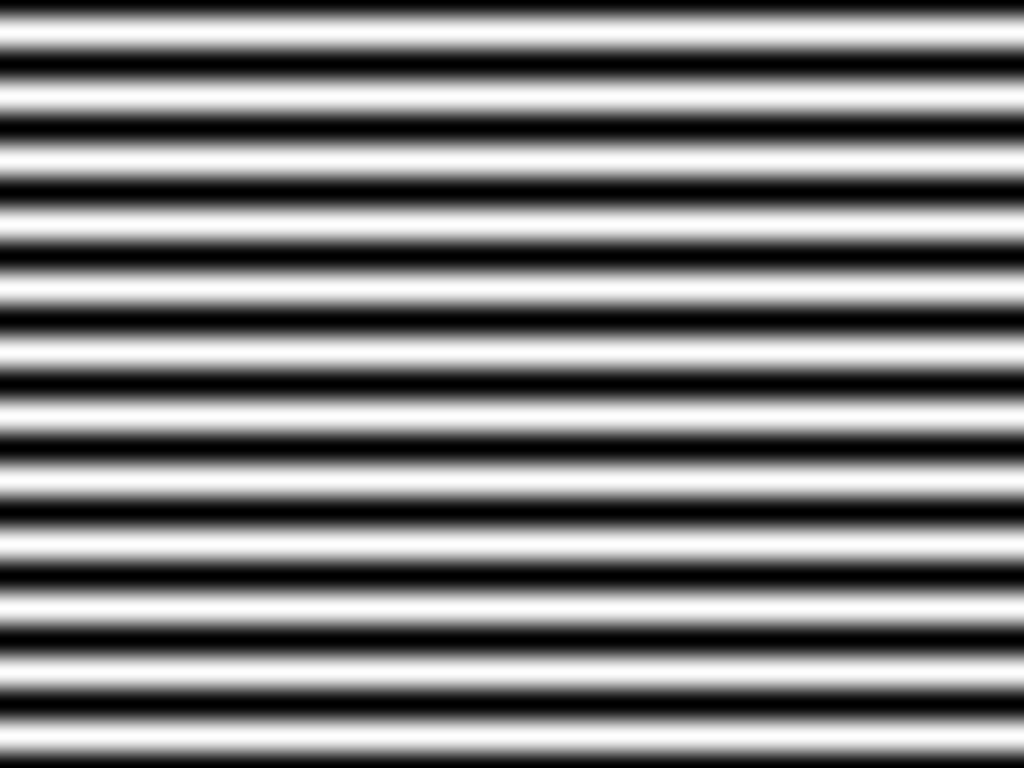
\includegraphics[width=5cm,height=5cm]{../img_source/phase_hor_1.jpg}}
\node at (0.0,-3) {\color{red} Projector image};
\pgftext[at=\pgfpoint{6cm}{0cm}]{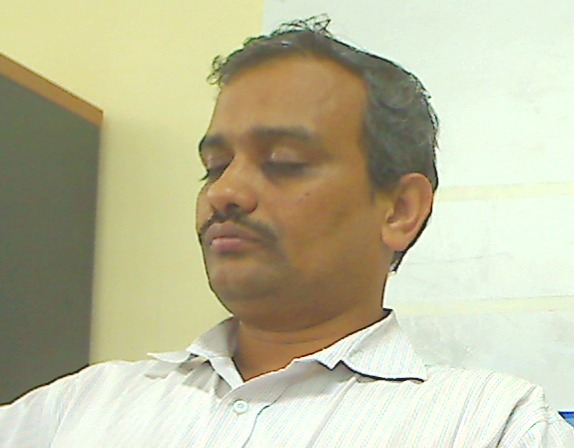
\includegraphics[width=5cm,height=5cm]{../img_source/face_2d.jpg}}
\node at (6,-3){\color{red} Camera image};
\pgftext[at=\pgfpoint{3cm}{9cm}]{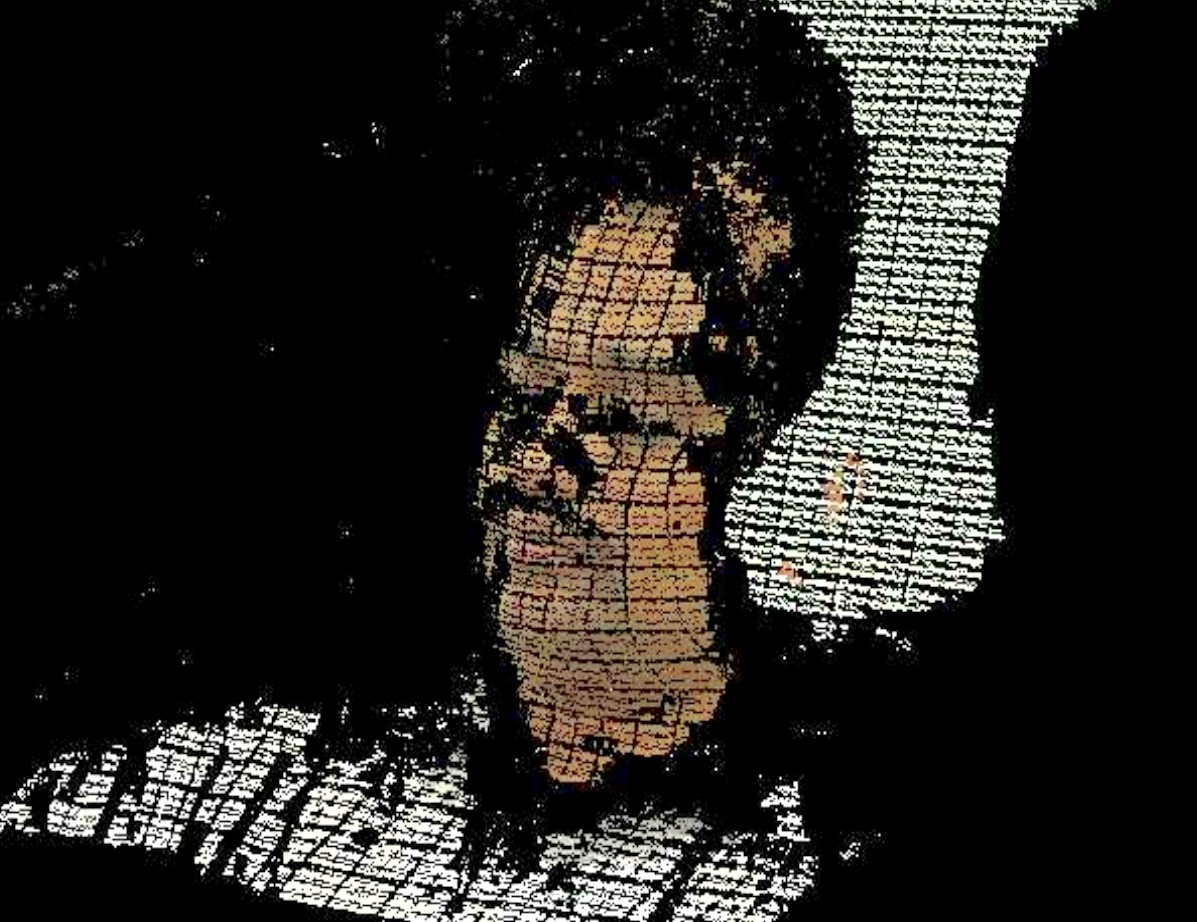
\includegraphics[width=5cm,height=5cm]{../img_source/face_3d.jpg}}
\node at (3,12){\color{red} Real-world object};
\draw [->](0,0)--(3.2,8);
\draw [->](3.2,8)--(6.1,-.7);
\draw[.] (6,0);
\fill [green] (3.2,8) circle[radius=2pt];
\fill [green] (6.1,-.7) circle[radius=2pt];
\fill [green] (0.0,0.0) circle[radius=2pt];
\end{tikzpicture}
\caption{Stereo correspondence and triangulation}
\label{fig:correspond_triangulate}
\end{figure}
\FloatBarrier
In figure~\ref{fig:correspond_triangulate}, a point in \textit{Projector image} is related to a point in \textit{Camera image} because they are 2D projections of a common point in the scene using the estimated stereo-correspondence. Once system is calibrated, ray-ray intersection between optical ray of camera and that of corresponding projector pixel gives the (X,Y,Z) coordinates of real-world point in \textit{physical unit} like `mm', `m' etc. \newline

\indent Figure~\ref{fig:arch} graphically represents the layout of our 3D scanner system, which can be referred during thesis. Working of \textbf{\textit{System calibration module}} is documented in chapter-2. \textbf{\textit{Pattern generation, Pattern projection and capture, Phase wrapper, Phase unwrapper, Absolute phase computation modules}} are explained in chapter-3. \textbf{\textit{Triangulation module}} has been described in chapter-4. 

\begin{figure}[!h]
\centering
\begin{tikzpicture}
  [node distance=2.0cm,
  start chain=going below,]
     \node[punktchain, join] (intro) {Pattern generation};
     \node[punktchain, join] (probf)      {Pattern projection and capture};
     \node[punktchain, join] (investeringer)      {Phase wrapping};
     \node[punktchain, join] (perfekt) {Phase unwrapping};
     \node[punktchain,join] (emperi) {Absolute phase computation};
\node[punktchain,join](triangulate){\textbf{\textit{Triangulation}}};
\begin{scope}[start branch=x,every join/.style={->,thick,shorten <=1pt},]
\node[punktchain,on chain=going left,join=by {<-},node distance=-14.0cm](calib) {\textbf{\textit{System calibration}}};
\end{scope}

\draw[tuborg, decoration={brace}] let 
  \p1=(intro.north), \p2=(emperi.south) in 
   ($(2.3, \y1)$) -- ($(2.3,\y2)$) node[tubnode] {\textbf{\textit{Stereo correspondence}}};

\node at (-1.8,-1.5) {\textit{Generated patterns}};

\node at (-1.7,-4.8){\textit{Captured patterns}};

\node at (-1.5,-8.1){\textit{Wrapped phase}};

\node at (-1.7,-11.4){\textit{Unwrapped phase}};

\node at (-3.1,-14.7){\textit{Camera-projector correspondence}};

\node[above] at (4.5,-16.5){\textit{camera,projector}}; 
\node[below] at (4.6,-16.4){\textit{calibration parameters}};
\end{tikzpicture}
\caption{Architecture of the developed system}
\label{fig:arch}
\end{figure}



\chapter{System calibration} 
 
         
For performing non-metric reconstruction only point-to-point correspondences between camera and projector are needed to perform triangulation[3]. But to relate the depth computed using triangulation with physical metrics such as 'mm', 'cm' etc there is need to relate the camera and projector geometry with physical measurement units, this task is accomplished by process of System calibration.  Calibration is a process of determining intrinsic and extrinsic characteristics of the imaging devices(camera and projector in our case). Intrinsic characteristics include focal length, coordinates of principal points of lens used in camera and projectors, image axis skew coefficients and lens distortion coefficients. Extrinsic characteristics include rigid-body transformations that can transform a point represented in World-coordinate system to individual coordinates systems of camera and projector. \newline 

 
Above discussion clearly implies the need to establish defining equations which relate a real-world three dimensional point(with coordinates expressed in \textit{physical} units) with pixel coordinates in camera(or projector). For this purpose a projective model of camera which applies to projector as well is introduced in the next section which clearly describes the problem of calibration, following which the current approaches and the approach used in this work to solve this problem will be reviewed. In the end, a note on \textit{relative extrinsic calibration} of projector-camera system is mentioned, which is a process of determining relative rotation and translation of camera and projector coordinate systems which in simple words means to determine the relative orientation and position of camera with respect to projector or vice-versa.   
  
\section{Camera model}   
Camera model is a concise mathematical abstraction of the internal(i.e., its optics and sensor arrangement) and external(i.e., its position relative to a scene) geometry of camera which is responsible for the imaging process. In this section, these geometric parameters will be described and hence the imaging process. Camera model described here is referred from seminal paper by [8]. Other calibration techniques also follow variants of this formulation. Relatively recent work in [9] has shown projector to be \textit{inverse-camera} hence further discussion on camera calibration holds equally to projector as well. Section 2.4.2 will describe how  projector was calibrated similar to camera with a real example. In next subsection the coordinate-systems which are relevant for geometric modeling of imaging process under consideration will be described.  
  
\subsection{Graphical abstraction}  
In this subsection the graphical model of camera depicting coordinate systems involved in transforming a real world 3D point to camera 2D coordinate representation will be described.
   
\paragraph{World-coordinate system.}  
World-coordinate system defines the reference frame in the real world that will be used for defining the positions of object in scene in physical units. Typically any location in the real scene can be used as origin for world coordinate system axes. For example in this work world coordinate system origin was assumed to be present at a corner on a wall.  
  
\paragraph{Camera-coordinate system.}  
This is a 3D reference coordinate-system internal to camera, it is similar to world coordinate system since it also works in physical units. Its origin is assumed to be at center of projection of camera. It is used to generate 3D interpretation of the scene from camera viewpoint.  
  
\paragraph{Image-coordinate system.}  
This is a 2D reference coordinate-system for indexing points in the real-image. Note here \textit{real} means that it can take real values as coordinates. It is used to index the points in perspective projection of 3D world.  
  
\paragraph{Computer-frame coordinate system.}  
This is a 2D reference coordinate-system which indexes pixels in the computer-frame. It can only have integral coordinates. Images with which we normally interact are indexed with respect to this coordinate system. \newline  
  
Figure~\ref{fig:coordinate_systems}\footnote{Figure source: Refer~\cite{8}} illustrates the coordinate systems except computer-frame coordinate system since it is not geometrically connected with other coordinate systems:  
  
%\begin{figure}[hb]  
%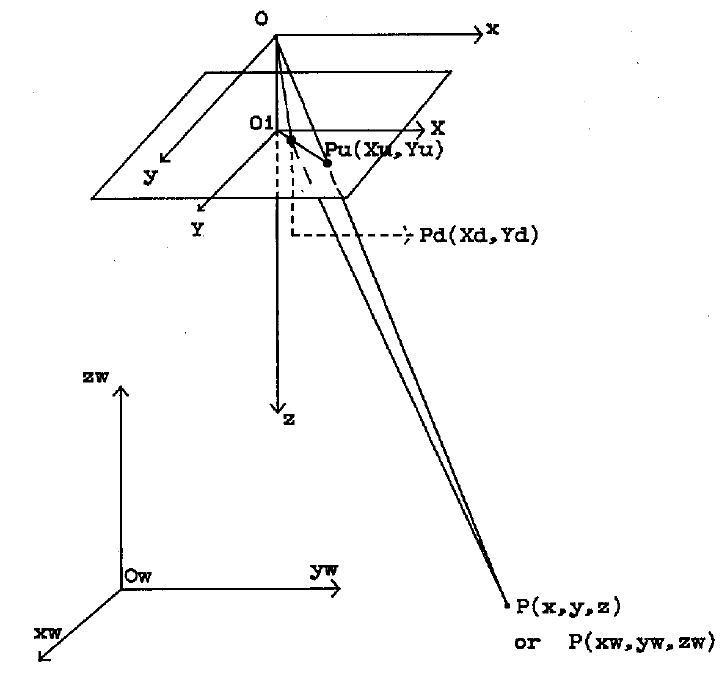
\includegraphics[width=10cm,height=10cm]{../img_source/coordinate_systems.jpg}  
%\caption{Transformation of a real world 3D point from world coordinate system to computer-buffer coordinate system}  
%\label{fig:coordinate_systems}
%\end{figure}  

\begin{figure}[ht]
\centering
\begin{tikzpicture}
% world coordinate system
\draw[->] (0,0)--(0,3);%Y
\draw[->] (0,0)--(3,0);%X
\draw[->] (0,0)--(-1.5,-1.5);%Z
\node[below] at (0,0) {\textbf{$O_w$}};
\node[below] at (3,0) {\textbf{$X_w$}};
\node[left] at (0,3) {\textbf{$Y_w$}};
\node[below] at (-1.0,-1.5) {\textbf{$Z_w$}};

% camera coordinate system
\draw[->] (2,9)--(2,4);%Z
\draw[->] (2,9)--(5,9);%X
\draw[->] (2,9)--(1,6);%Y
\node[left] at (2,9) {\textbf{$O_c$}};
\node[above] at (5,9) {\textbf{$X_c$}};
\node[below] at (2,4) {\textbf{$Z_c$}};
\node[below] at (1,6) {\textbf{$Y_c$}};

% camera-image coordinate system
\draw (0.5,8)--(6,8);
\draw (0.5,8)--(-0.5,6);
\draw (6,8)--(5,6);
\draw (-0.5,6)--(5,6);

\node[left] at (2,7.5) {\textbf{$O_i$}};
\fill [black] (2,7.5) circle[radius=2pt];

\draw[->] (2,7.5)--(4,7.5);
\draw[->] (2,7.5)--(1,4.5);
\node[below] at (4,7.5){\textbf{$X_i$}};
\node[left] at (1,4.5){\textbf{$Y_i$}};

%3d point
\node[below] at (7,-1){\textbf{$P$}};
\fill [black] (7,-1) circle[radius=2pt];

\draw (7,-1)--(2.9,7.3);
\fill[black] (2.9,7.3) circle[radius=2pt];
\node[below] at (2.9,7.3) {\textbf{$P_u$}};

\draw (2.9,7.3)--(2,9);


\node[below] at (2.5,6.9) {\textbf{$P_d$}};
\fill[black] (2.5,6.9) circle[radius=2pt];

\draw (7,-1)--(2.5,6.9);
\draw (2.5,6.9)--(2,9);

\end{tikzpicture}
\caption{Transformation of a real world 3D point from world coordinate system to computer-buffer coordinate system}  
\label{fig:coordinate_systems}
\end{figure}  


Here points $O_w,O_c$ and $O_i$ represent origins of world,camera and real-image coordinate systems respectively. Further, axes $X_w,Y_w$ and $Z_w$ represent the world-coordinate system, axes $X_c,Y_c$ and $Z_c$ denote the camera coordinate system, similarly axes $X_i$ and $Y_i$ show the 2D real-image coordinate system, $P$ is a real-world point, $P_u$ is the ideal projection of $P$ on real-image plane(i.e., image-coordinate system), $P_d$ is corresponding distorted projection which differ from $P_u$ due to practical imperfections in camera system. Equations relating these coordinate systems are described in the following paragraphs of this section.  
  
\subsection{Mathematical abstraction}  
In this subsection, the actual mathematical form of camera imaging process which is used for transforming a real-world 3D point to a computer-buffer pixel will be sequentially described. This involves a series of coordinate transformations which are described here.   

\paragraph{1.Rigid body transformations from object world-coordinate system to camera coordinate system.}  
Points in the world-coordinate coordinates system (x\textsubscript{w},y\textsubscript{w},z\textsubscript{w}) are transformed to the camera-coordinate system (x\textsubscript{c},y\textsubscript{c},z\textsubscript{c}). To model this process, rotation(R) and translation(T) matrices are used as:  
  
\begin{equation}  
\begin{bmatrix}  
x_c \\  
y_c \\  
z_c  
\end{bmatrix}  
=  
R*   \begin{bmatrix}  
      x_w \\  
      y_w \\  
      z_w  
      \end{bmatrix}  
+T  
\end{equation}  
where $R=\begin{bmatrix}  
         r_{1,1} & r_{1,2} & r_{1,3} \\  
         r_{2,1} & r_{2,2} & r_{2,3} \\  
         r_{3,1} & r_{3,2} & r_{3,3}   
         \end{bmatrix}$  
,$T=\begin{bmatrix}  
    t_x \\  
    t_y \\  
    t_z  
   \end{bmatrix}$ \newline  
  
  
Rotation and translation parameters are called \textit{extrinsic parameters} of camera/projector. It should be noted here that rotation followed by translation is used since it ensures unique transformations, whereas translation followed by rotation can result in multiple possible transformations[8].  
  
  
  
\paragraph{2.Perspective transformation from camera-coordinates to real-image coordinates.}  
In this step, 3D scene as viewed from camera-coordinate origin is perspective projected to a plane. Hence it is a 3D to 2D transformation resulting in loss of Z-coordinate(i.e., depth) since multiple points are projected onto same point in the image-plane. Following equations describe this process:  
  
\begin{equation}  
\begin{bmatrix}  
x_u \\  
y_u  
\end{bmatrix}  
=\bigg(\frac{f}{z_c}\bigg)*  
\begin{bmatrix}  
x_c \\  
y_c  
\end{bmatrix}  
\end{equation}  
  
\noindent  
where \textit{f} represents the focal length of camera/projector lens. (x\textsubscript{u},y\textsubscript{u}) is the perspective projection of point (x\textsubscript{c},y\textsubscript{c},z\textsubscript{c}) on real-image plane.  
  
\paragraph{3.Radial and tangential lens distortion.}  
In this step, real-image coordinates are distorted due to radially imperfections in practical lens which is characterized by \textit{radial distortion} and oblique alignment of principal plane of lens and sensor-plane which is characterized by \textit{tangential distortion}. Although Tsai's work only accounted for radial distortions subsequent works have accounted for tangential[10] and prism distortions[11] also in an attempt to increase the accuracy of estimated calibration parameters further. Following equations describes the effect of radial and tangential distortion on \textit{ideal} image coordinates:  
\begin{equation}  
\begin{aligned}
& x_d=x_u(1+k_1r^2+k_2r^4+k_3r^6+...)+2p_1x_uy_u+p_2(r^2+2x_u) \\
& y_d=y_u(1+k_1r^2+k_2r^4+k_3r^6+...)+2p_2x_uy_u+p_1(r^2+2y_u)
\end{aligned}
\end{equation}  
\noindent  
where,\newline
$(x_d,y_d)$: distorted image coordinates\newline
$(k_1,k_2,k_3)$: radial distortion coefficients\newline
$(p_1,p_2)$: tangential distortion coefficients\newline
$r=\sqrt[2]{X_u^2+Y_u^2}$
  
\paragraph{4.Transforming real-image coordinates to computer-frame coordinates.}  
Finally to map 3D world-coordinates to frame coordinates of camera, i.e., the pixels that we see, following equations are assumed:  
\begin{equation}  
\begin{bmatrix}  
x_f \\  
y_f  
\end{bmatrix}  
=\begin{bmatrix}  
s_x*(d_x^{'})^{-1}*x_d\\  
d_y^{-1}*y_d  
\end{bmatrix}   
+\begin{bmatrix}  
C_x \\  
C_y  
\end{bmatrix}  
\end{equation}  
\noindent  
where,\newline  
$(x_f,y_f)$:computer frame-buffer coordinates for point $(x_d,y_d)$ \newline  
$s_x$:uncertainty image-scale factor \newline  
$d_x$:center-to-center distance between sensor cells along X-direction\newline  
$N_{cx}$:Number of sensors along X-direction\newline  
$N_{fx}$:Number of pixels along X-line sampled by computer\newline  
$d_x^{'}=d_x*\left(\frac{N_{cx}}{N_{fx}}\right)$\newline\newline  
It should be noted that at full camera resolution there is one-to-one relation between number of sensor elements and number of pixels in computer-frame buffer hence $N_{cx}=N_{fx}$ and hence $d_x^{'}=d_x$ but in general $d_x^{'}>=d_x$. [8] attributed $s_x$ to be due to  possibility of mismatch between camera image acquisition hardware and camera scanning hardware. Figure~\ref{fig:cam_model_pipeline}\footnote{Figure source: Refer~\cite{8}} illustrates the complete imaging process. 
%\begin{figure}[ht]  
%\centering  
%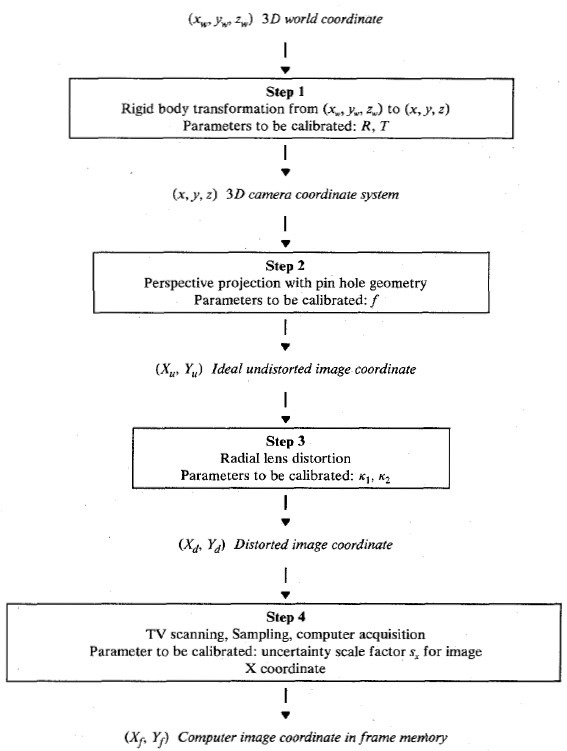
\includegraphics[width=10cm,height=14cm]{../img_source/cam_model_pipeline.jpg}  
%\caption{Camera model pipeline}  
%\label{fig:cam_model_pipeline}
%\end{figure}  
\begin{figure}
\centering
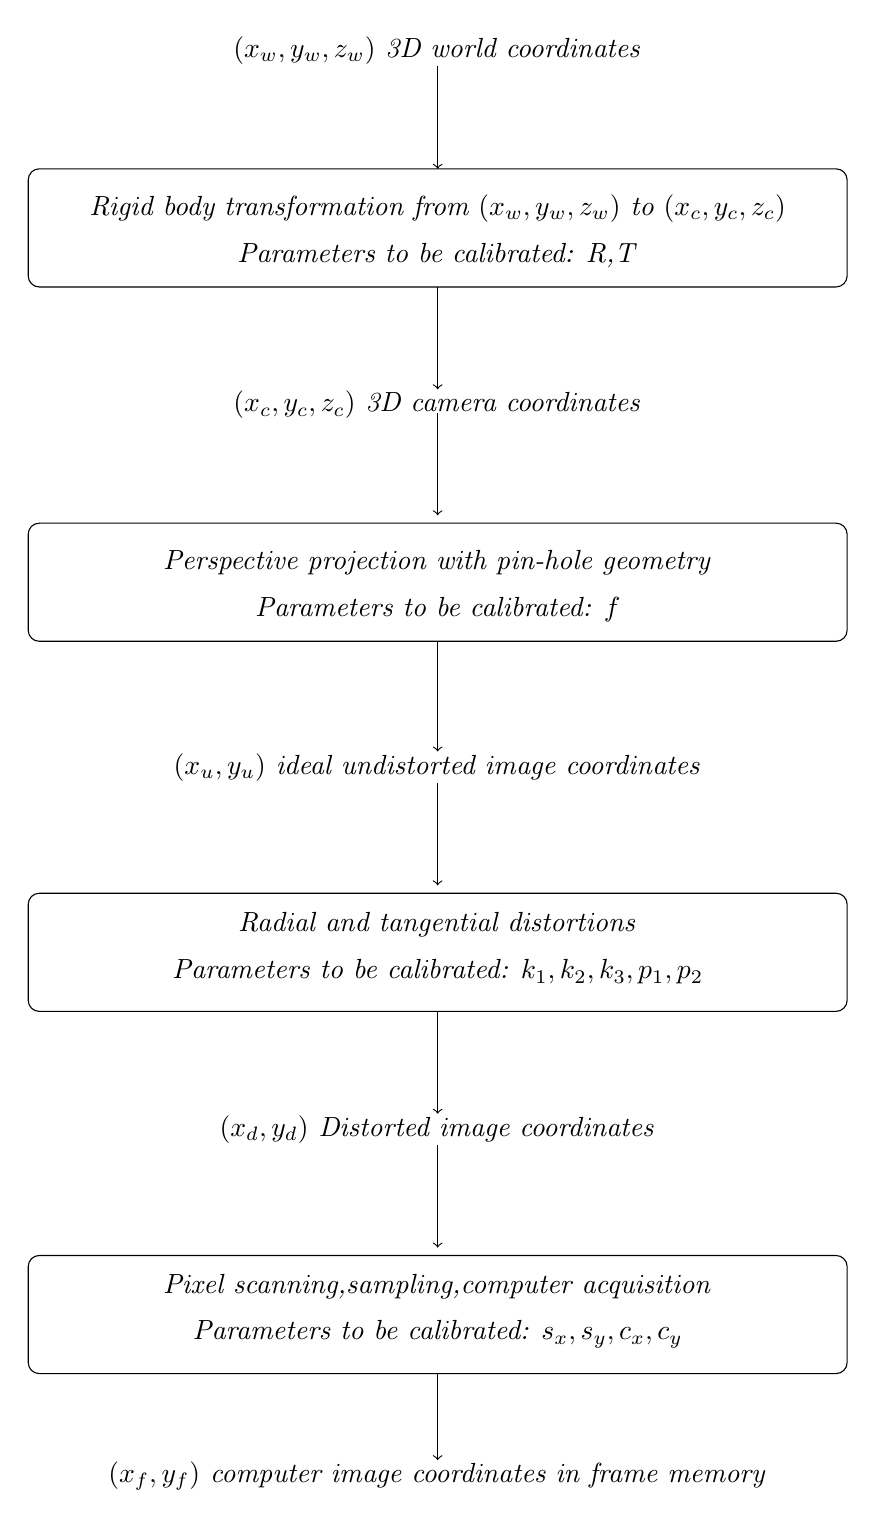
\begin{tikzpicture}
\node at (0,0) {\textit{$(x_w,y_w,z_w)$ 3D world coordinates}};
\draw[->] (0,-0.2)--(0,-1.5);
\draw[rounded corners] (-5.2,-1.5) rectangle (5.2,-3);
\node at (0,-2.0){\textit{Rigid body transformation from $(x_w,y_w,z_w)$ to $(x_c,y_c,z_c)$}};
\node at (0,-2.6) {\textit{Parameters to be calibrated: R,T}};

\draw[->] (0,-3)--(0,-4.3);
\node at (0,-4.5) {\textit{$(x_c,y_c,z_c)$ 3D camera coordinates}};
\draw[->] (0,-4.6)--(0,-5.9);
\draw[rounded corners] (-5.2,-6.0) rectangle (5.2,-7.5);
\node at (0,-6.5) {\textit{Perspective projection with pin-hole geometry}}; \node at (0,-7.1) {\textit{Parameters to be calibrated: $f$}};

\draw[->] (0,-7.5)--(0,-8.9);
\node at (0,-9.1) {\textit{$(x_u,y_u)$ ideal undistorted image coordinates}};

\draw[->] (0,-9.3)--(0,-10.6);
\draw[rounded corners] (-5.2,-10.7) rectangle (5.2,-12.2);
\node at (0,-11.1) {\textit{Radial and tangential distortions}};
\node at (0,-11.7) {\textit{Parameters to be calibrated: $k_1,k_2,k_3,p_1,p_2$}};

\draw[->] (0,-12.2)--(0,-13.5);
\node at (0,-13.7) {\textit{$(x_d,y_d)$ Distorted image coordinates}};
\draw[->] (0,-13.9)--(0,-15.2);
\draw[rounded corners] (-5.2,-15.3) rectangle (5.2,-16.8);

\node at (0,-15.7) {\textit{Pixel scanning,sampling,computer acquisition}}; 
\node at (0,-16.3) {\textit{Parameters to be calibrated: $s_x,s_y,c_x,c_y$}};

\draw[->] (0,-16.8)--(0,-17.9);
\node at (0,-18.1) {\textit{$(x_f,y_f)$ computer image coordinates in frame memory}};
\end{tikzpicture}
\caption{Camera model pipeline}  
\label{fig:cam_model_pipeline}
\end{figure}

\noindent  
So based on above discussion we can deduce that to define the geometric imaging process of camera(or projector) we have to estimate following parameters:
\begin{enumerate}  
\item Internal parameters:
\begin{enumerate}
\item Camera lens focal length
\item Position of principal point on the real-image plane
\item Lens distortion parameters
\end{enumerate}
\item External parameters:
\begin{enumerate}
\item Rotation between camera-coordinate system and world-coordinate system  
\item Translation between camera-coordinate system and world-coordinate system  
\end{enumerate}
\end{enumerate}  
  
  
  
\section{Current approaches:A review}  
A taxonomy was proposed by [10] for camera calibration approaches based on their requirement of additional calibration objects as:  
\paragraph{a) Photogrammetric calibration.}  
These techniques perform camera calibration by observing a calibration object. Calibration object can be any object with known geometry i.e., we know world-coordinates of feature-points on the object that we want to use for calibration. In this category many techniques for both 3D and 2D calibration objects were proposed. For example use of 3D calibration object with three orthogonal planes or planar calibration rigs with known translation across its views have been used for calibration[8] although requiring elaborate setup for calibration and often time-consuming.  
\paragraph{b) Self-calibration.}  
These techniques are more flexible than photogrammetric techniques in that they do not require an explicit calibration rig for calibration, but by moving the camera across a static rigid scene they determine constraints on internal parameters of camera that can be used for calibration[12][13]. Other than these techniques there are techniques that do not fall into these categories
such as camera calibration using vanishing points for orthogonal directions[14], calibration from pure rotation[15]. In this work, a photogrammetric method for camera and projector calibration was used. Following paragraphs will briefly describe the details of some highly cited and practically used algorithms in chronological order.\newline  
  
\paragraph{R.Y.Tsai's algorithm.}  
Tsai's algorithm restricts the lens-distortion effects to only radial distortion and do not account for skewness or lack of orthogonality of projection. Calibration was divided in 2 separate stages. In first stage all extrinsic parameters except for $t_z$ are computed using the \textit{Radial alignment constraint(RAC)} shown in figure~\ref{fig:rac}\footnote{Figure source: Refer~\cite{16}}. If assumed lens distortion is only \textit{radial}, then the direction of vector $O_iP_d$ remains unchanged and is parallel to vector $P_{oz}P_w$. Tsai showed that RAC is independent of magnitude of effective focal length, radial distortion coefficients and position of point $P_w$ along z-axis. He further proved that this constraint is sufficient to estimate 3D rotation and translation of $P_w$ along X and Y axes. \newline   
\begin{figure}[ht]  
\centering  
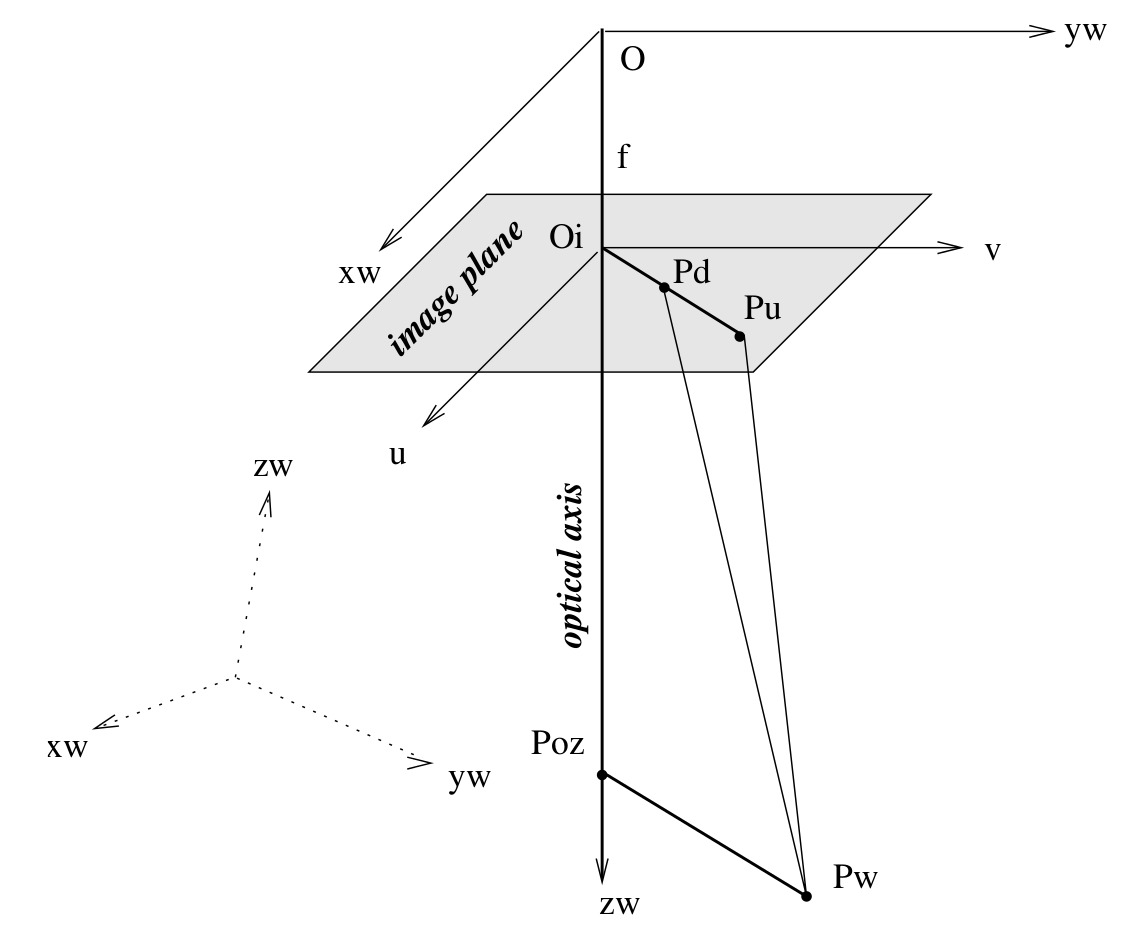
\includegraphics[width=13cm,height=10cm]{../img_source/tsai_rac.jpg}  
\caption{Radial alignment constraint used in Tsai's algorithm}  
\label{fig:rac}
\end{figure}  
  
\noindent  
In second stage effective focal length, distortion coefficients and $t_z$ are estimated using non-linear optimization.  
  
  
\paragraph{Z.Zhang's algorithm.}  
Z.Zhang proposed a plane based camera calibration algorithm[10]. It first acquires real-world coordinate to camera image coordinate correspondences using planar calibration board. Then it estimates all intrinsic and extrinsic parameters using a closed-form solution. This closed form solution assumes zero lens distortion and is based on two constraints on intrinsic parameters derived from the \textit{orthonormality} of rotation vector expressed in equations 2.5,2.6.  
\begin{equation}  
h_1^TA^{-T}A^{-1}h_2=0  
\end{equation}  
\begin{equation}  
h_1^TA^{-T}A^{-1}h_1=h_2^{T}A^{-T}A^{-1}h_2  
\end{equation}  
\noindent  
where,\newline  
$h_i$: $i^{th}$ column vector of Homography\newline  
$A$: Camera projective matrix\newline  
  

Further, the coefficients of radial distortion $k_1,k_2$ are estimated by solving linear least squares expressed in equation 2.7.  
\begin{equation}  
\begin{bmatrix}  
(u-u_0)(x^2+y^2) & (u-u_0)(x^2+y^2)^2 \\  
(v-v_0)(x^2+y^2) & (v-v_0)(x^2+y^2)^2  
\end{bmatrix}  
\begin{bmatrix}  
k_1 \\  
k_2  
\end{bmatrix}  
=\begin{bmatrix}  
u'-u \\  
v'-v  
\end{bmatrix}  
\end{equation}\newline  
\noindent  
where,\newline  
$(u,v)$: ideal pixel image coordinates\newline  
$(u_0,v_0)$: coordinates of principal point\newline  
$(x,y)$: ideal normalized image coordinates\newline  
  

\noindent  
Estimated values of all parameters are considered as initial input for non-linear least squares minimization which minimizes expression in equation 2.8.  
\begin{equation}  
\sum_{i=1}^{m}\sum_{j=1}^{n}||m_{ij}-m'(A,k_1,k_2,R_i,t_i,M_j)||^2  
\end{equation}\newline  
\noindent  
where,\newline  
$m$: Total number of features on the calibration board \newline  
$n$: Total number views of planar calibration board \newline  
$M_j$: 3D coordinates of $j^{th}$ feature point on calibration board\newline  
$m_{ij}$: True 2D coordinates of projection of $M_j$ in camera image\newline   
$m'$: Estimated 2D coordinates for $M_j$ using calibration parameters\newline  
$R_i$: Rotation parameters for $i^{th}$ view used for calibration\newline  
$t_i$: Translation parameters for $i^{th}$ view used for calibration\newline  
  
\paragraph{J.Heikkila et al.'s algorithm.}  
This algorithm assumes a more elaborate camera model which includes both radial and tangential components as lens distortion coefficients. It first linearizes the camera model by ignoring lens distortion coefficients and performs linear parameter estimation using Direct Linear Transformation(DLT)[17]. Equation 2-9 shows the linear model solved using DLT method.\newline  
\begin{equation}  
La=0  
\end{equation}\newline  
\noindent  
where,\newline   
a=$\begin{bmatrix}  
a_{1,1} & a_{1,2} & a_{1,3} & a_{1,4} & a_{2,1} & a_{2,2} & a_{2,3} & a_{2,4} & a_{3,1} & a_{3,2} & a_{3,3} & a_{3,4}   
\end{bmatrix}$\newline  
\newline  
L=$\begin{bmatrix}  
X_1 & Y_1 & Z_1 & 1 & 0 & 0 & 0 & 0 & -X_1u_1 & -Y_1u_1 & -Z_1u_1 & -u_1 \\  
0 & 0 & 0 & 0 & X_1 & Y_1 & Z_1 & 1 & -X_1v_1 & -Y_1v_1 & -Z_1v_1 & -v_1 \\    
: & : & : & : &  :  &  :  &  :  & : &   :     &    :    &    :    &   : \\  
X_i & Y_i & Z_i & 1 & 0 & 0 & 0 & 0 & -X_iu_i & -Y_iu_i & -Z_iu_i & -u_i \\  
0 & 0 & 0 & 0 & X_i & Y_i & Z_i & 1 & -X_iv_i & -Y_iv_i & -Z_iv_i & -v_i \\  
: & : & : & : &  :  &  :  &  :  & : &   :     &    :    &    :    &   : \\  
X_n & Y_n & Z_n & 1 & 0 & 0 & 0 & 0 & -X_nu_n & -Y_nu_n & -Z_nu_n & -u_n \\  
0 & 0 & 0 & 0 & X_n & Y_n & Z_n & 1 & -X_nv_n & -Y_nv_n & -Z_nv_n & -v_n   
\end{bmatrix}$ \newline  
\newline  
\newline  
\noindent  
Here, $(X_i,Y_i,Z_i)$ denotes 3D coordinates of $i^{th}$ feature point used in calibration, $(u_i,v_i)$ denotes the corresponding 2D image coordinates, \textit{a} denotes the projective matrix mapping $(X_i,Y_i,Z_i)$ to $(u_i,v_i)$.  
In second step, Gaussian noise model is assumed and a non-linear least square minimization is performed to minimize equation 2-10.\newline    
\begin{equation}  
F=\sum_{i=1}^N\big[(U_i-u_i)^2+(V_i-v_i)^2\big]  
\end{equation}  
\noindent  
where, \textit{N} is the number of observations, $(U_i,V_i)$ are the observed 2D coordinates of $i^{th}$ feature point, $(u_i,v_i)$ are corresponding 2D coordinates estimated using calibration parameters.  
  
  
  
\section{Approach followed in this work}  
For camera and projector calibration an extension of [10] method was used which was first described and developed in [18] and later ported to OpenCV. Unfortunately, author in [18] has not published the details of algorithm except describing the approach to be based on camera model described in [17] and implementation as a variant of [10] hence  
OpenCV documentation other than reading the source code itself is the only source of  
theoretical information on this technique. During this project work, an effort is initiated  
to fully understand the calibration algorithms and effect of each calibration  
parameters on accuracy of 3D reconstruction by actually implementing an algorithm  
so that every input to the algorithm can be changed and its effect seen. For which technique described in [17] was selected and partially implemented. Here a brief outline of camera/projector calibration algorithm implemented in OpenCV/Matlab[18][19] is presented:  
\begin{enumerate}
\item A planar calibration board is selected with known world-coordinates of reference points on it.  
\item Calibration board is shown for multiple views(at least 2) in front of camera by varying its rotation and translation(amount need not be known) with respect to camera and for every pose feature-points are  
detected in camera.  
\item After all such views are captured and feature-points detected, homography for each view is calculated.  
\item Closed form solution of intrinsic parameters from homographies using orthogonality of vanishing points is computed but unlike [10] no initial estimates of distortion coefficients are computed.  
\item Initial estimates of calibration parameters computed earlier are given as input to Maximum likelihood estimator Levenberg-Marquardt algorithm[20] to refine the parameters.Output of this process is a set of calibration parameters which optimally satisfy the maximum likelihood criteria.  
\end{enumerate}

 
\paragraph{Algorithm for extrinsic calibration of camera and projector.}  
Extrinsic parameters relate camera-coordinate system and projector-coordinate system to world-coordinate system. For  
extrinsic calibration, OpenCV[21] performs minimization of re-projection error between  
observed point projections given as input(i.e., image points) and projection computed  
by applying the estimated model to the given object points. Extrinsic parameters that  
minimize this criteria are considered as the optimal pose(Rotation and translation)  
parameters.  
  
\paragraph{A note on Relative calibration of projector and camera.}  
After camera and projector are calibrated extrinsically, there is need to relate their  
coordinate-systems with each other so that a point in projector coordinate-system can  
also be expressed in terms of camera-coordinate system. This is required because of  
an implicit assumption in triangulation is that it requires intersection of optical rays from  
camera and projector, which is possible only if we can express both rays in a common  
coordinate-system either in that of camera or projector. This is achieved  
using our world-coordinate system as a common link between projector and camera.  
Following equations relate camera-coordinate system to projector-coordinate system  
via world-coordinate system[22]:  
\begin{equation}  
\begin{bmatrix}  
P_c \\  
P_p  
\end{bmatrix}  
=\begin{bmatrix}  
R_{wc}*P_w \\  
R_{wp}*P_w  
\end{bmatrix}  
+\begin{bmatrix}  
T_{wc} \\  
T_{wp}  
\end{bmatrix}  
\end{equation}  
hence,\newline  
$P_c=\underbrace{(R_c*R_p^{-1})}_{R_{pc}}*P_p+\underbrace{(T_c-R_c*R_p^{-1}*P_p)}_{T_{pc}}$  
  
\noindent  
where,\newline  
$P_w$:A point in world coordinate system\newline  
$P_c$:Representation of $P_w$ with respect to camera coordinate system\newline  
$P_p$:Representation of $P_w$ with respect to projector coordinate system\newline  
$R_{wc}$:Rotation transformation from world-to-camera coordinate system\newline  
$R_{wp}$:Rotation transformation from world-to-projector coordinate system\newline  
$T_{wc}$:Translation transformation from world-to-camera coordinate system\newline  
$T_{wp}$:Translation transformation from world-to-projector coordinate system\newline  
$R_{pc}$:Rotation transformation from projector-to-camera coordinate system\newline  
$T_{pc}$:Translation transformation from projector-to-camera coordinate system\newline  
  
Here $R_{pc}$ and $T_{pc}$ are the final outcomes which allows us to map a point in projector coordinate system to camera coordinate system which is an requirement for performing stereo-triangulation.  
  
\section{Working of developed system calibration module}  
System calibration is composed of camera calibration, projector calibration and relative extrinsic calibration of camera with respect to projector. A module for system calibration was developed which performs above mentioned functions using OpenCV camera calibration and extrinsic calibration algorithms. This section first describes the system setup and then explains the practical procedure for camera, projector and extrinsic calibration of projector with respect to camera.  
  
\paragraph{System setup.}  
In this work,Logitech Quickcam sphere AF web-cam at 1600X1200 pixels  
resolution was as a capture device, Sharp PG-F200X projector at 1024X768 pixels resolution was used for pattern projection, and 4 markers(shown in figure~\ref{fig:calib_setup} as `black' points) as world coordinate references forming a  
rectangular region of 1900mm X 1700mm and a physical checkerboard with square  
size 25.6mm arranged in a 10X8 square grid. Figure~\ref{fig:calib_setup} shows setup of our 3D  
scanner system:\newline  
  
\begin{figure}[htbp]  
\centering  
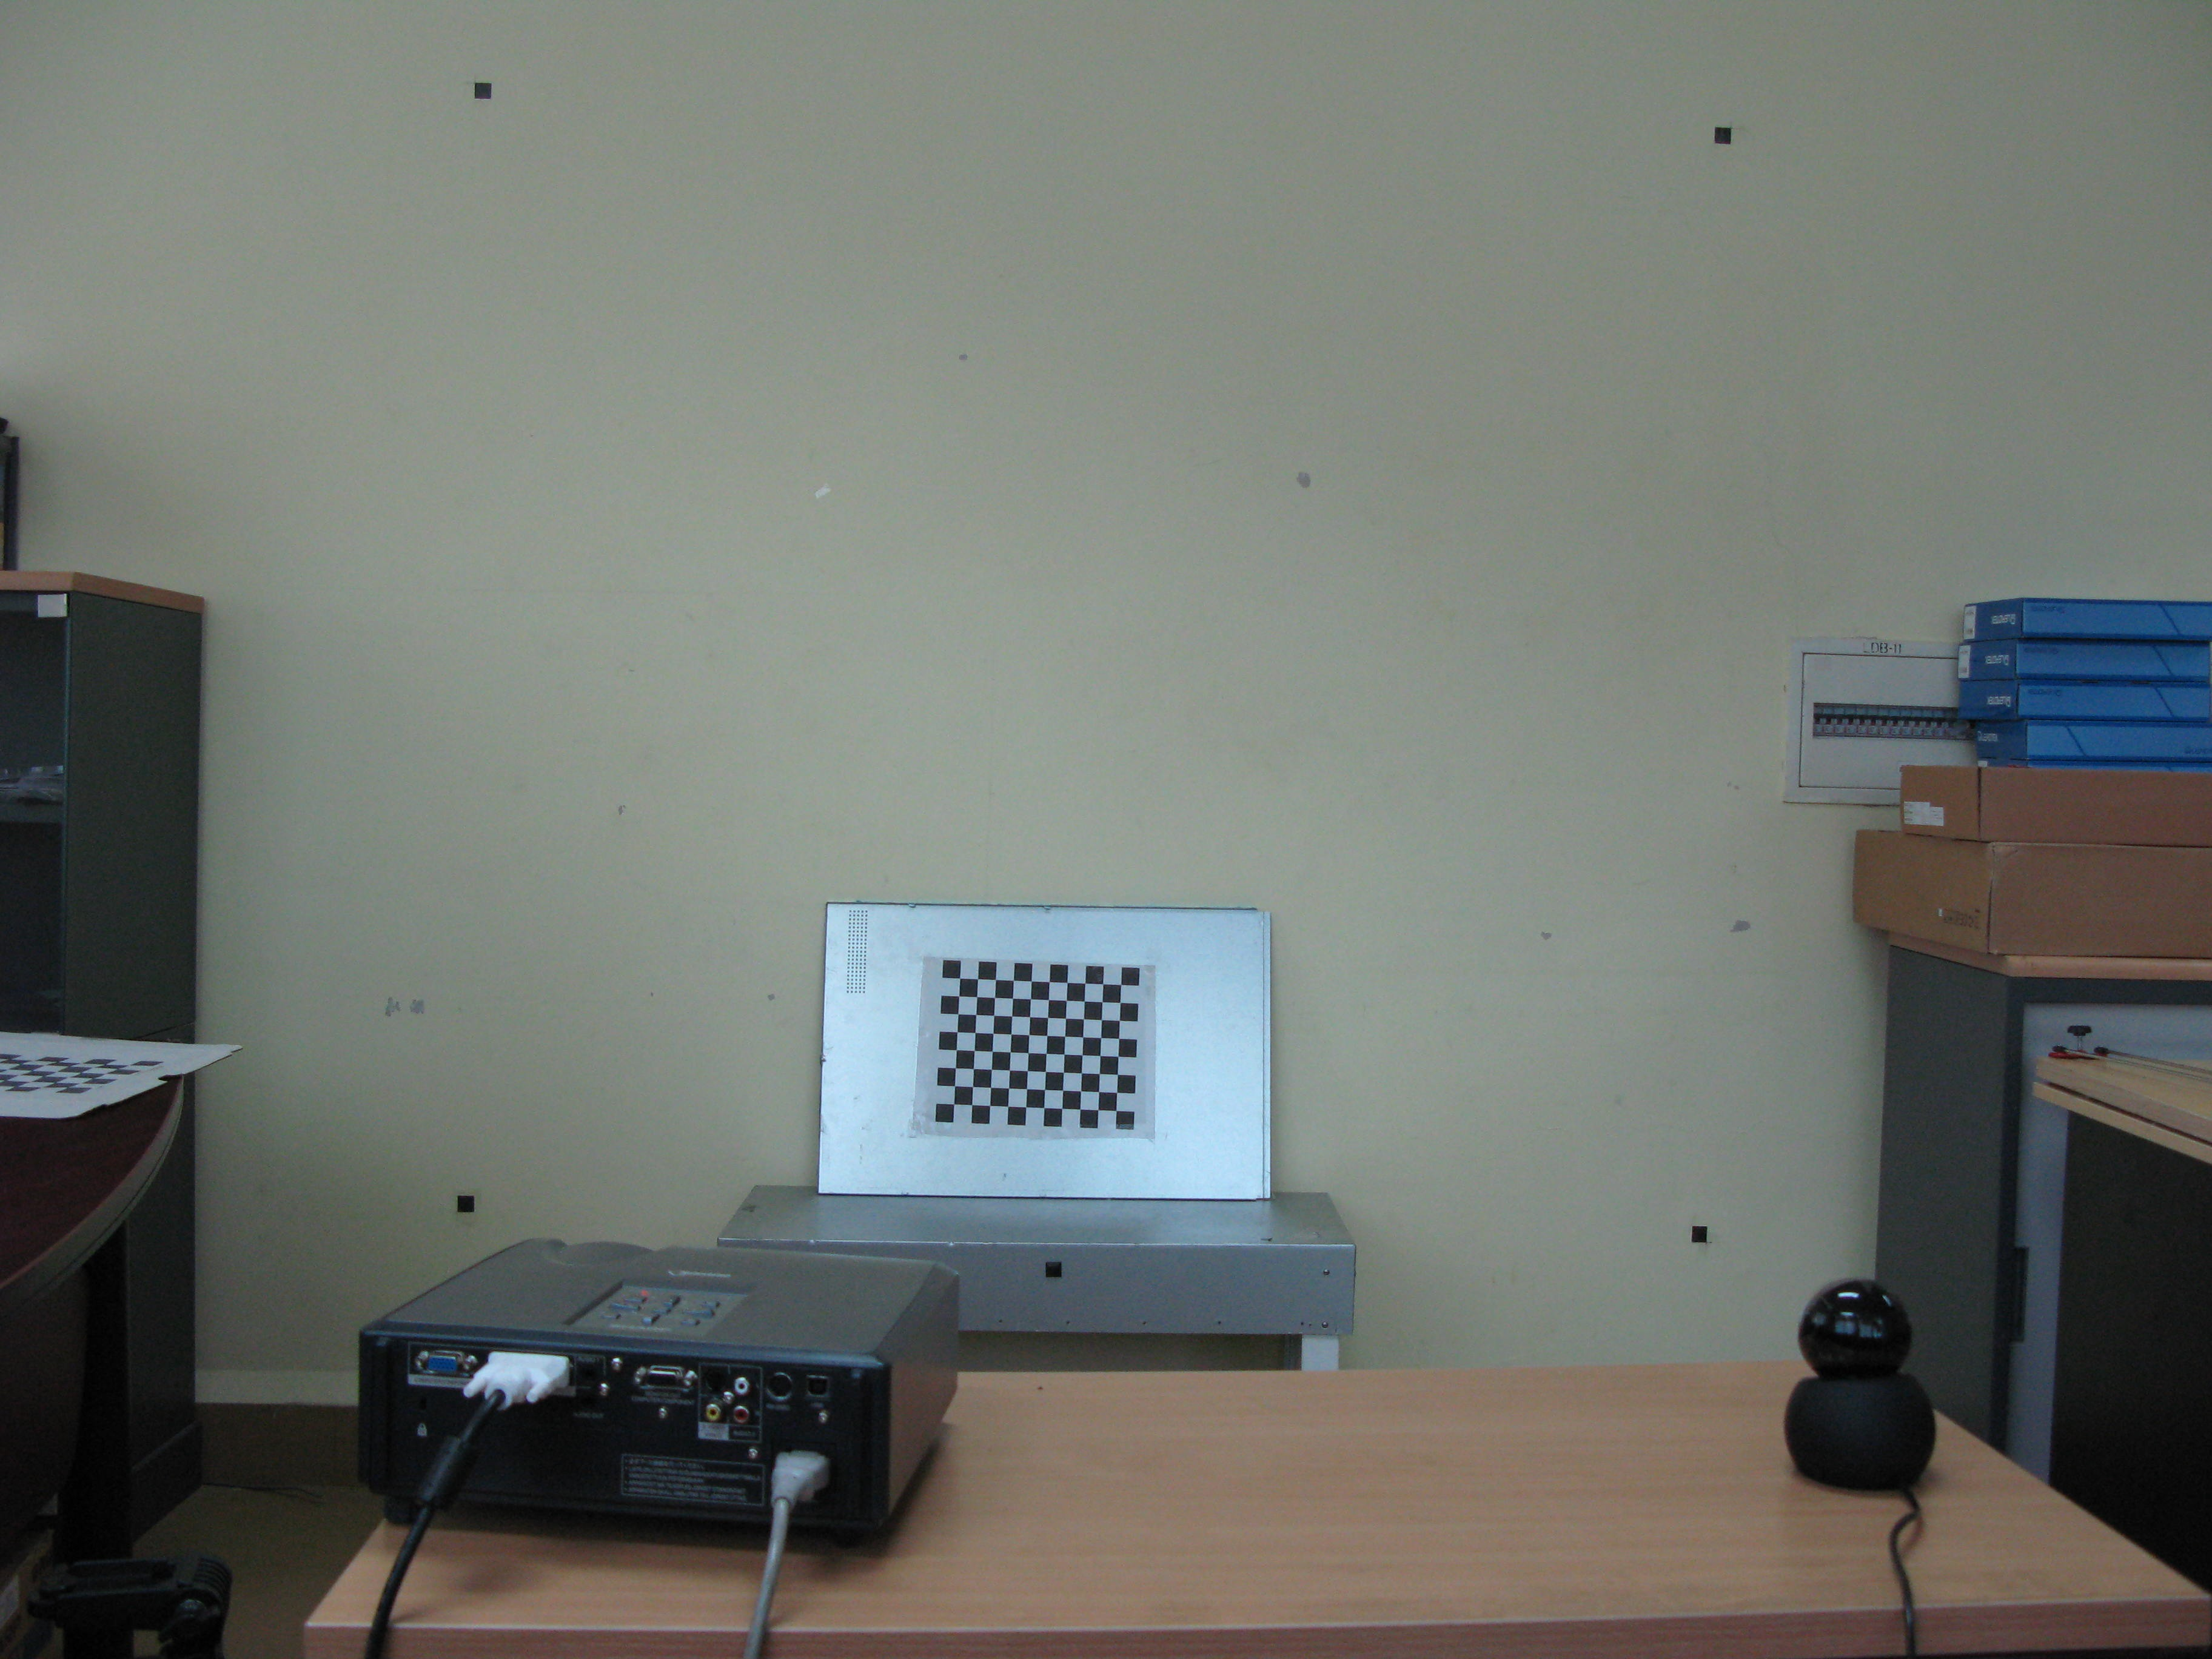
\includegraphics[width=10cm,height=8cm]{../img_source/system_setup.jpg}  
\caption{System setup}
\label{fig:calib_setup}  
\end{figure}  
  
\subsection{Camera calibration}  
In this work, camera calibration was performed using OpenCV camera calibration function whose theoretical foundations were laid by the well known algorithms by [10] and [17]. Basic overview of algorithm was presented in Section-2.3.OpenCV estimates 9 intrinsic parameters to define internal geometry of camera and 6 extrinsic parameters to define external geometry of camera with respect to world coordinate system.\newline  
\textbf{Intrinsic and distortion parameters}\newline  
$f_x$: focal length of camera lens expressed in number of pixels along X - axis\newline  
$f_y$: focal length of camera lens expressed in number of pixels along Y - axis\newline  
$(c_x , c_y)$: Pixel coordinates of principal point\newline  
$(k_1, k_2, k_3)$: Radial distortion coefficients\newline  
$(p_1,p_2)$: Tangential distortion coefficients\newline  
\textbf{Extrinsic parameters}\newline  
$(r_x,r_y,r_z)$: Rotation vector between camera and world coordinate system\newline  
$(t_x,t_y,t_z)$: Translation vector between camera and world coordinate system  
\paragraph{Procedure:}  
Aim of this process is to acquire 3D-2D correspondences between world coordinate  
system and camera image coordinate system which are then used to estimate intrinsic and  
extrinsic parameters of camera. World coordinate system origin is assumed to be at top-left corner  
of the physical checkerboard although it can be at any arbitrary position. Please note that this coordinate system origin is different from the world coordinate origin used for measurement(i.e., a corner on wall) described earlier.\newline  
\noindent  
Multiple views of the checkerboard are captured by camera and inner corners are  
detected with sub-pixel accuracy. Figure~\ref{fig:cam_calib_views} shows some such views used.\newline  
\begin{figure}[htbp]  
\centering  
\def\tabularxcolumn#1{m{#1}}  
\begin{tabularx}{\linewidth}{@{}cXX@{}}  
\begin{tabular}{c c c c}  
\hspace{0.8cm}
\subfloat[]{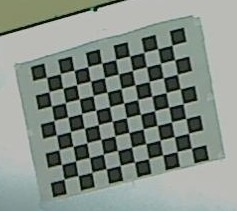
\includegraphics[width=3cm,height=3cm]{../img_source/cam_1.jpg}} &  
\subfloat[]{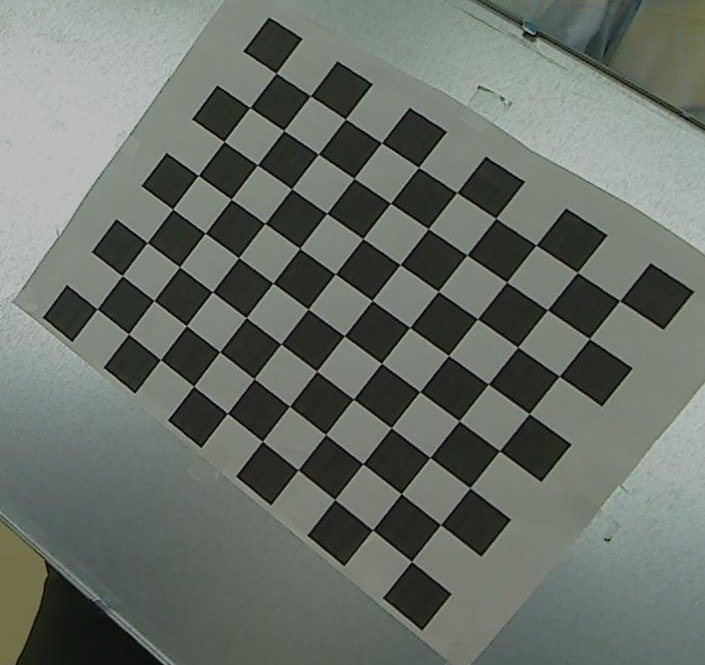
\includegraphics[width=3cm,height=3cm]{../img_source/cam_2.jpg}} &  
\subfloat[]{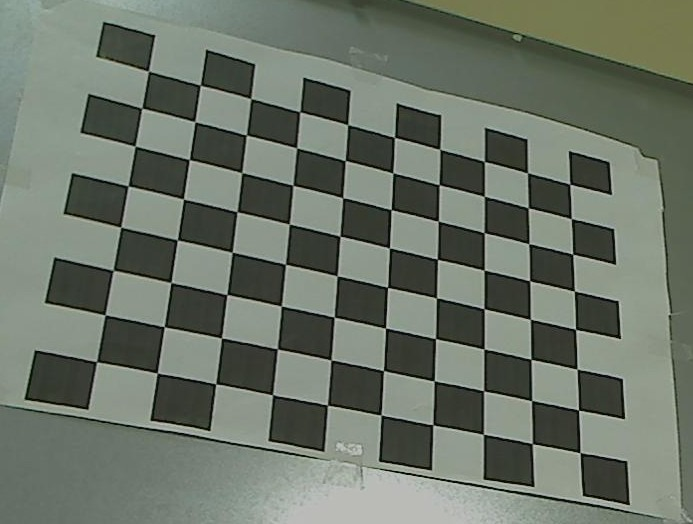
\includegraphics[width=3cm,height=3cm]{../img_source/cam_3.jpg}} &  
\subfloat[]{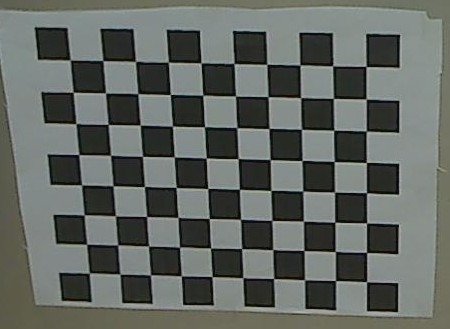
\includegraphics[width=3cm,height=3cm]{../img_source/cam_4.jpg}}\\  
\end{tabular}  
\end{tabularx}  
\caption{Some views used for camera calibration}  
\label{fig:cam_calib_views}
\end{figure}  
Each such view provides a set of 3D-2D correspondence and adds a separate set of rotation and translation parameters to the  
list of unknowns. Since there are 15 unknowns parameters per view hence at least 15 equations needs to be solved for the unknowns. This requires at least 2 views since a single view can provide only 8 constraints(i.e., 4 points are required to completely define a homography). Practically, we use more than 2 views(typically greater than 10) with more than  
4 points per view to account for effect of noise in corner-detection. Acquired 3D-2D point  
correspondences are used to calibrate camera as explained in Section-2.3.  
  
\paragraph{Results and visualization.}  
For visualization of camera calibration process a program to plot the  
views used for calibration was developed. This visualization is similar to [18] but it was not available  
for projector calibration.\newline  
Figures~\ref{fig:cam_calib_plot_1},~\ref{fig:cam_calib_plot_2} show snapshots of 3D plot of all views of checkerboard used for camera  
calibration.  
\noindent  
Here, figure~\ref{fig:cam_calib_plot_1} shows that our calibration range was 50cm to 250cm along Z-axis, -25cm to +45cm along Y-axis.  
\begin{figure}[htbp]  
\centering  
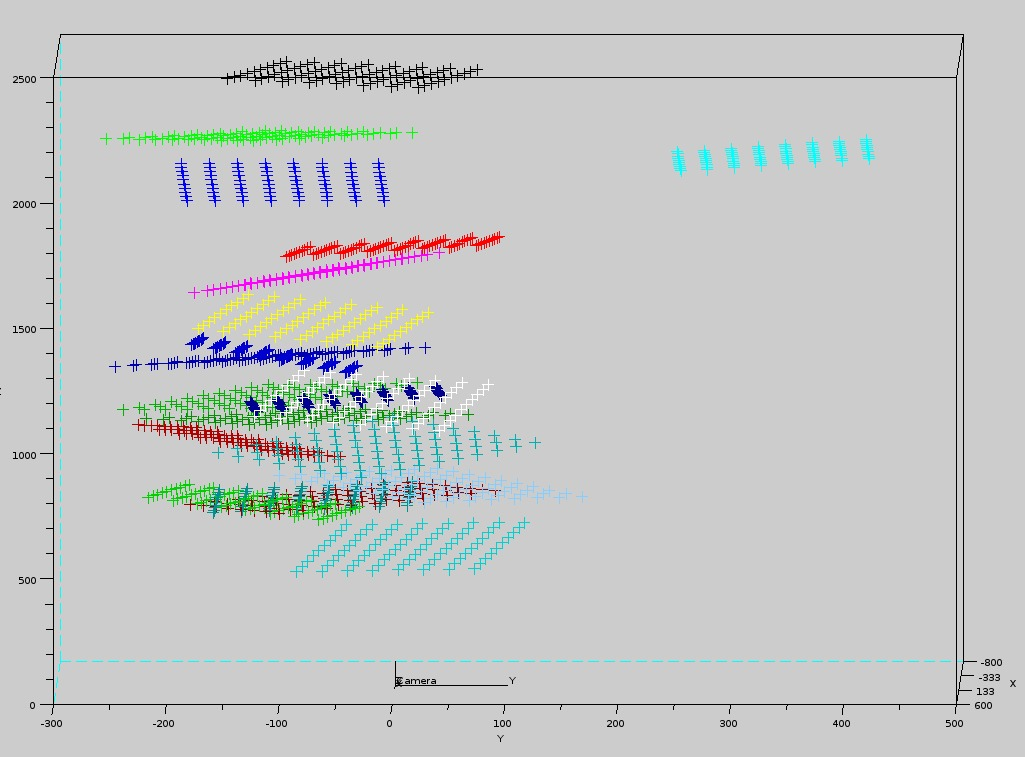
\includegraphics[width=15cm,height=10cm]{../img_source/cam_calib_view.jpg}  
\caption{Visualization of camera calibration results:View along X-axis}  
\label{fig:cam_calib_plot_1}
\end{figure}  
\noindent  
Figure~\ref{fig:cam_calib_plot_2} shows that calibration range along X-axis  
was -50cm just above +40cm. All above mentioned distances are with respect to  
camera coordinates system, which is at (0,0,0) in both figures. So the camera  
calibration volume was approximately 90cm X 70cm X 200cm.  
\begin{figure}[htbp]  
\centering  
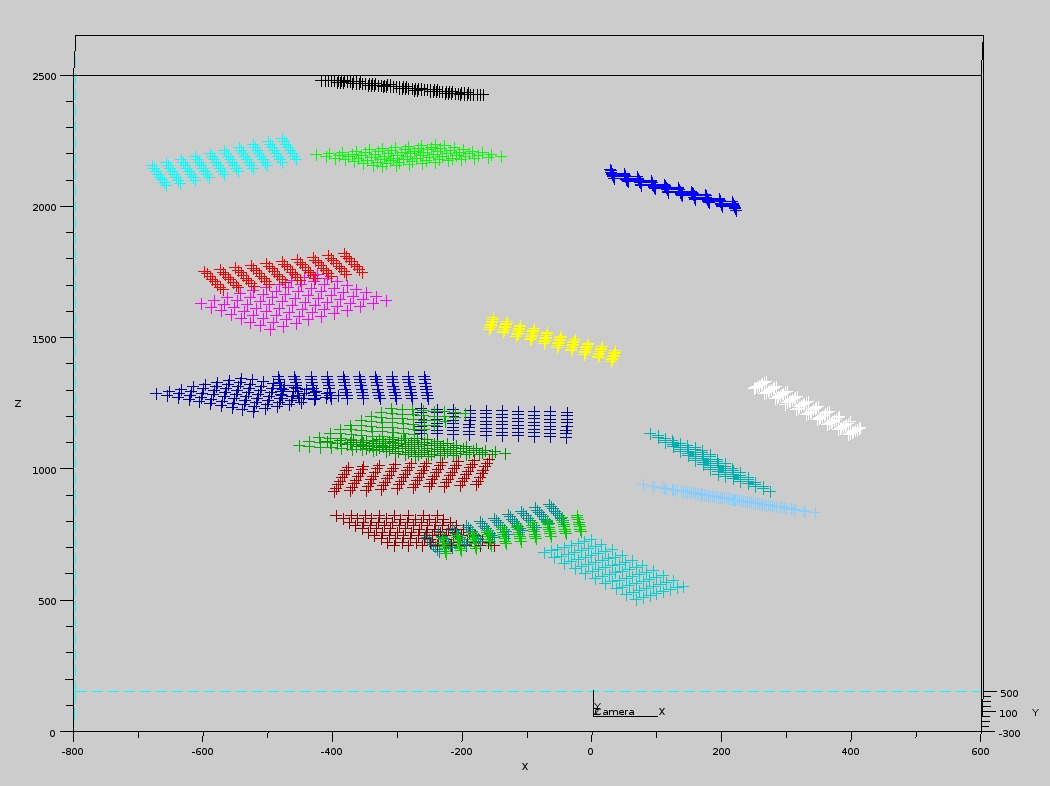
\includegraphics[width=15cm,height=10cm]{../img_source/cam_calib_view2.jpg}  
\caption{Visualization of camera calibration results:View along Y-axis} 
\label{fig:cam_calib_plot_2} 
\end{figure}  
Camera calibration parameters estimated through experiments for Logitech Quickcam sphere AF webcam at native resolution are tabulated in table 2-1. \textit{Reprojection error} mentioned in the table can be defined as a measure of deviation of fitted parameters from the observed world-camera point correspondences.% More formally,  
%\paragraph{Reprojection error.}  
%A measure of accuracy of fitted camera parameters. This is a geometric error, which quantitatively represents the euclidean distance between actual projection of a 3D point(the detected corners) and its projection computed using the estimated parameters.
\begin{table}[hb]  
\centering  
\begin{tabular}{c c}  
\hline\noalign{\smallskip}  
Parameter & Estimated value \\  
\noalign{\smallskip}\hline\noalign{\smallskip}  
$f_x$ & 1362.2\\  
$f_y$ & 1372.2\\  
$c_x$ & 803.9\\  
$c_y$ & 590.1\\  
$k_1$ & 0.07\\  
$k_2$ & -0.14\\  
%$k_3$ & 0.0\\  
%$p_1$ & 0.0\\  
%$p_2$ & 0.0\\  
Reprojection error & 0.20 \\  
\noalign{\smallskip}\hline  
\end{tabular}  
\caption{Estimated Camera intrinsic and distortion model parameters}  
\end{table}   
\subsection{Projector calibration}  
As already mentioned in Section-2.1, projector calibration problem can be regarded as an inverse-camera calibration problem. Consequently, same procedure as of camera calibration has been used to calibrate the projector. Basically, the idea is to use camera as a feedback device which will provide the 3D coordinates for the 2D features projected by the projector, hence providing the 3D-2D point correspondence between world-coordinate system and projector-coordinate system needed for projector calibration similar to camera calibration process.  
  
\paragraph{Procedure:}  
\begin{enumerate}
\item Camera-to-world homography is computed once.
\item For each view,
\begin{enumerate}
\item Projector is physically displaced allowing for rotations and translation with respect to world coordinate system and a checkerboard pattern is projected.  
\item Camera captures the projected features and detects their coordinates. 
\item Using camera-to-world homography, corresponding 3D coordinates are computed.  
\item These 3D coordinates along with the 2D coordinates of projected features(in projector buffer) forms the required 3D-2D correspondence for this view. 
\end{enumerate}
\item After sufficient number of such views(typically greater than 10) are captured projector calibration is performed using same algorithm as for camera calibration.  
\end{enumerate}
  
\noindent   
Figure~\ref{fig:proj_calib_view} shows few views used for projector calibration, projected checkerboard pattern has board dimension 11 squares X 9 squares and has each square of size of 75 pixels X 75 pixels.  
  
\begin{figure}[htbp]  
\centering  
\def\tabularxcolumn#1{m{#1}}  
\begin{tabularx}{\linewidth}{@{}cXX@{}}  
\begin{tabular}{c c c c}  
\hspace{0.8cm}  
\subfloat[]{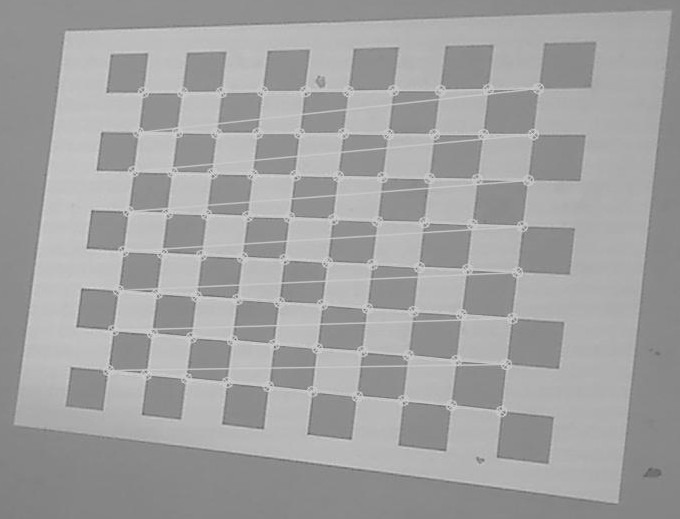
\includegraphics[width=3cm,height=3cm]{../img_source/proj_view_1.jpg}} &  
\subfloat[]{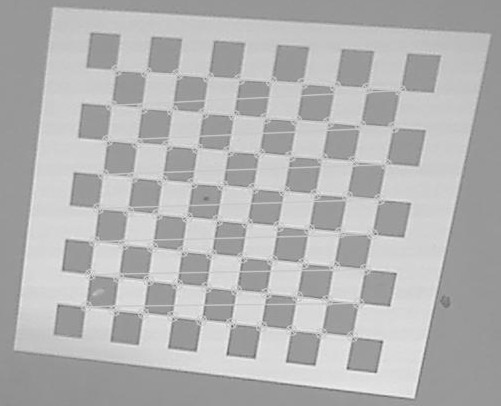
\includegraphics[width=3cm,height=3cm]{../img_source/proj_view_2.jpg}} &  
\subfloat[]{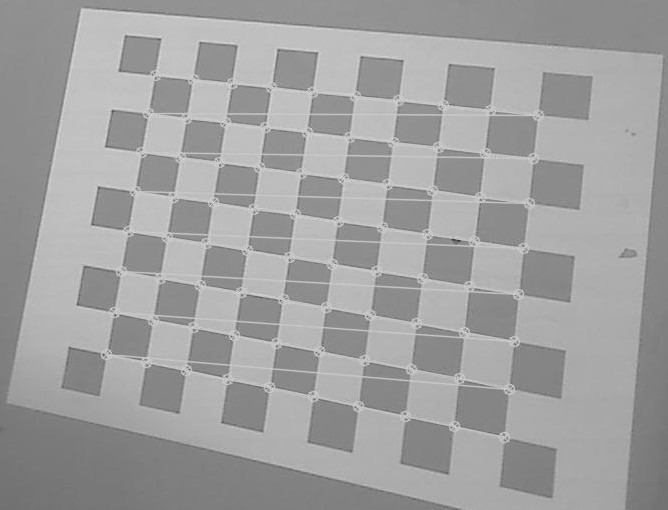
\includegraphics[width=3cm,height=3cm]{../img_source/proj_view_3.jpg}} &  
\subfloat[]{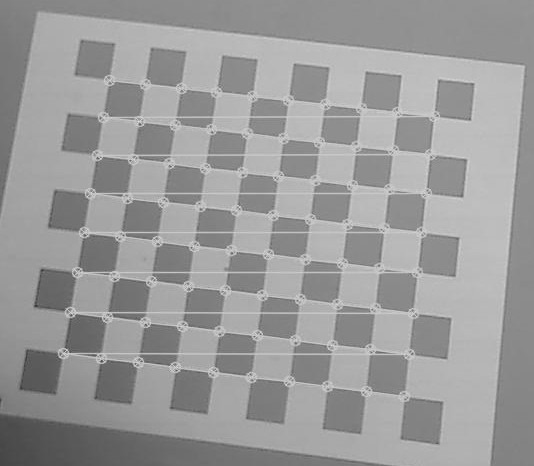
\includegraphics[width=3cm,height=3cm]{../img_source/proj_view_4.jpg}} \\  
\end{tabular}  
\end{tabularx}  
\caption{Some view used for projector calibration} 
\label{fig:proj_calib_view} 
\end{figure}  
  
  
\paragraph{Results and visualization.}  
Calibration parameters for Sharp PG F200X projector computed by performing above mentioned procedure are tabulated in table 2.2.  
\begin{table}[htbp]  
\centering  
\begin{tabular}{c c}  
\hline\noalign{\smallskip}  
Parameter & Estimated value \\  
\noalign{\smallskip}\hline\noalign{\smallskip}  
$f_x$ & 2261.7\\  
$f_y$ & 2262.8\\  
$c_x$ & 522.7\\  
$c_y$ & 713.8\\  
%$k_1$ & 0.0\\  
%$k_2$ & 0.0\\  
%$k_3$ & 0.0\\  
%$p_1$ & 0.0\\  
%$p_2$ & 0.0\\  
\noalign{\smallskip}\hline  
\end{tabular}  
\caption{Estimated Projector intrinsic model parameters}  
\end{table}  
\noindent  
Figures~\ref{fig:proj_calib_plot_1}, ~\ref{fig:proj_calib_plot_2} show plots of views used for projector calibration.Here, figure~\ref{fig:proj_calib_plot_1} shows that calibration range for along X-axis is -100cm to +150cm along Z-axis it is -50cm to +250cm.  
\begin{figure}[htbp]  
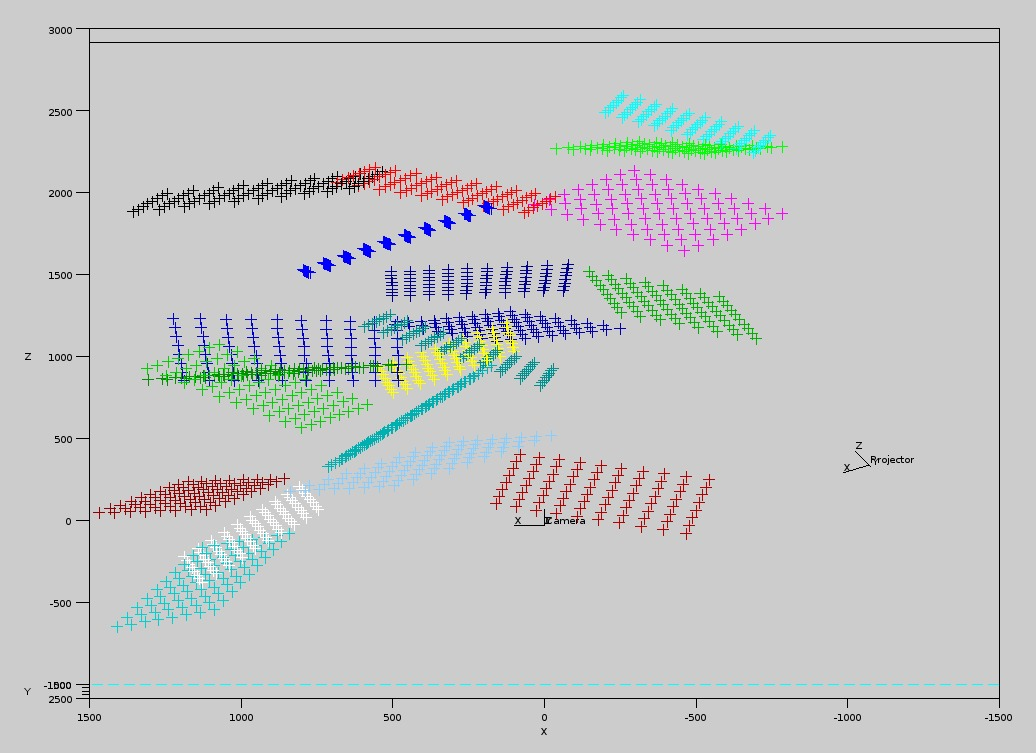
\includegraphics[width=15cm,height=10cm]{../img_source/proj_calib_plot_1.jpg}   
\caption{Visualization of projector calibration views along Y-axis} 
\label{fig:proj_calib_plot_1} 
\end{figure}  
\noindent  
Figure~\ref{fig:proj_calib_plot_2} shows calibration range along Y-axis to be from -125cm to +225cm.All measurements are with respect to camera-coordinate system which is shown at (0,0,0) in the figures. Hence calibration volume for projector was 250cm X 400cm X 300cm.  
\begin{figure}[htbp]  
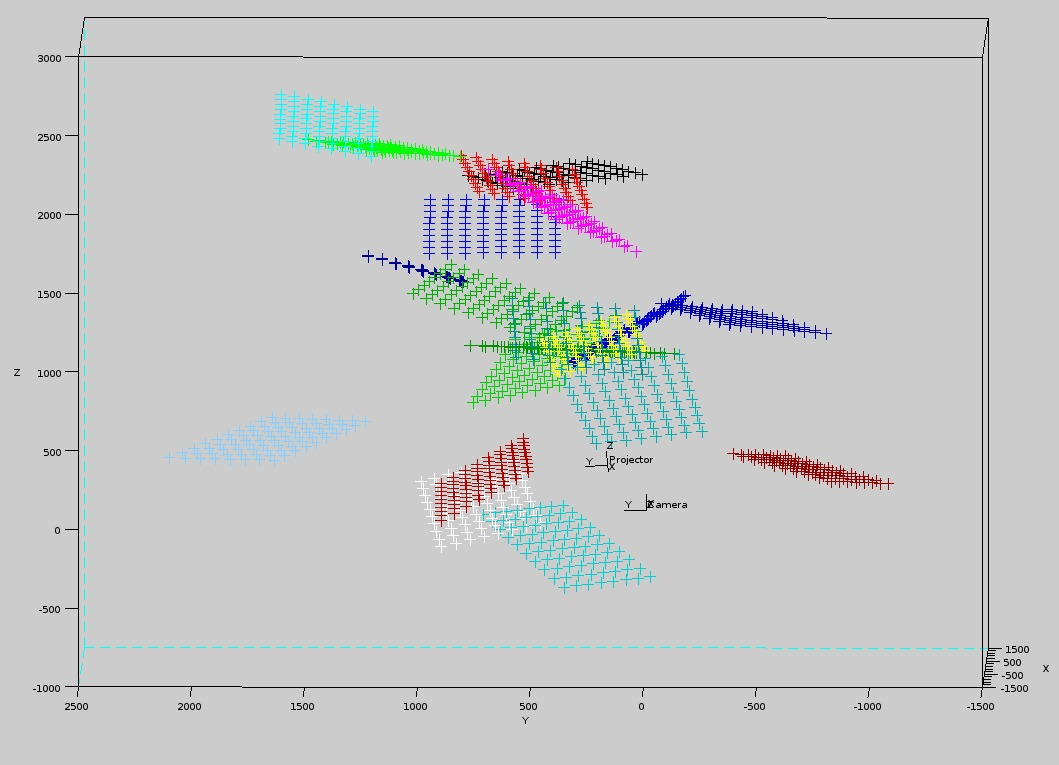
\includegraphics[width=15cm,height=10cm]{../img_source/proj_calib_plot_2.jpg}  
\caption{Visualization of projector calibration views along X-axis}  
\label{fig:proj_calib_plot_2}
\end{figure}  
  
  
  
  
  
\subsection{Camera-projector relative extrinsic calibration}   
As mentioned in an end note in section 2.3, relative calibration of projector with respect to camera is needed to bring both projector and camera to a common coordinate system which is a implicit assumption in triangulation. In this work, extrinsic calibration function available in OpenCV to determine the extrinsic parameters(i.e., rotation translation of projector coordinate system with respect to camera coordinate system) was used.  Rigid body transformations of camera and projector coordinate systems with respect to world coordinate system allow for determining the transformations between them(refer Note on relative calibration in section-2.3 for underlying equations)  
  
  
\paragraph{Procedure:}
\begin{enumerate} 
\item Extrinsic calibration of camera with respect to world coordinate system:  
\begin{enumerate}
\item A known reference plane(whose dimensions are known) containing world coordinate system is captured and corners are detected.  
\item These detected features are used for computing camera-to-world homography.  
\item Using the 3D-2D correspondences determined above, extrinsic calibration of camera is performed.  
\end{enumerate}
\item Extrinsic calibration of projector with respect to world coordinate system:  
\begin{enumerate}
\item Projector projects a checkerboard pattern, which is captured by the camera.  
\item Using the camera-to-world homography computed above, 3D coordinates for the projected feature points can be computed.  
\item These  3D-2D correspondences(3D coordinates of projected feature points and corresponding 2D coordinates in projector image) are used for computing relative rotation and translation of projector coordinate system with respect to world coordinate system.  
\end{enumerate}
\item Relative rotation and translation of projector coordinate system with respect to camera coordinate system is computed(refer Note on relative calibration in section 2.3 for underlying equations)  
\end{enumerate}  
  
\paragraph{Results and visualization.}  
Estimated extrinsic calibration parameters for a sample camera-projector geometry are tabulated in table 2.3,2.4,2.5.It should be noted however that these results are for one specific system configuration and do not represent any intrinsic characteristic of system. Hence they are called extrinsic parameters.\newline  

 
In tables~\ref{table:cam_extrinsics}.~\ref{table:proj_extrinsics},~\ref{table:cam_proj_extrinsics},  
$(r_1^{wc},r_2^{wc},r_3^{wc})$ is rotation transformation from world coordinate system to camera coordinate system  
$(t_1^{wc},t_2^{wc},t_3^{wc})$ is translation transformation from world coordinate system to camera coordinate system  
$(r_1^{wp},r_2^{wp},r_3^{wp})$ is rotation transformation from world coordinate system to projector coordinate system  
$(t_1^{wp},t_2^{wp},t_3^{wp})$ is translation transformation from world coordinate system to projector coordinate system  
$(r_1^{pc},r_2^{pc},r_3^{pc})$ is rotation transformation from projector coordinate system to camera coordinate system  
$(t_1^{pc},t_2^{pc},t_3^{pc})$ is translation transformation from projector coordinate system to camera coordinates system. Rotation vectors are expressed in radians in axis-angle form, translation is expressed in `mm'.\newline  
\begin{table}[ht]  
\parbox{.45\linewidth}{  
\centering  
\begin{tabular}{c c}  
\hline\noalign{\smallskip}  
Parameter & Estimated value \\  
\hline  
$r_1^{wc}$ & 0.128 \\  
$r_2^{wc}$ & 0.239 \\  
$r_3^{wc}$ & 0.035\\  
$t_x^{wc}$ & -920.7\\  
$t_y^{wc}$ & -834.6\\  
$t_z^{wc}$ & 2960.6\\  
\hline  
\end{tabular}   
\caption{Estimated camera extrinsic parameters}
\label{table:cam_extrinsics}
}  
\hfill  
\parbox{.45\linewidth}{  
\centering  
\begin{tabular}{c c}  
\hline\noalign{\smallskip}  
Parameter & Estimated value \\  
\hline  
$r_1^{wp}$ & -0.047 \\  
$r_2^{wp}$ & -0.246 \\  
$r_3^{wp}$ & 0.008\\  
$t_x^{wp}$ & -1054.0\\  
$t_y^{wp}$ & -1235.0\\  
$t_z^{wp}$ & 2281.0\\  
\hline  
\end{tabular}  
\caption{Estimated projector extrinsic parameters}  
\label{table:proj_extrinsics}
}\\  

\parbox{.45\linewidth}{
\centering  
\begin{tabular}{c c}  
\hline\noalign{\smallskip}  
Parameter & Estimated value \\  
\hline  
$r_1^{pc}$ & -0.086 \\  
$r_2^{pc}$ & 0.484 \\  
$r_3^{pc}$ & 0.006\\  
$t_x^{pc}$ & -1080.3\\  
$t_y^{pc}$ & 188.9\\  
$t_z^{pc}$ & 359.4\\  
\hline  
\end{tabular}  
\caption{Estimated projector-camera relative parameters}  
\label{table:cam_proj_extrinsics}
}  
\end{table}  
  
\noindent  
View used for extrinsic calibration of projector camera system is depicted in Figure~\ref{fig:extrinsic_calib_setup}. Figure~\ref{fig:extrinsic_plot} shows the plan-view of estimated projector-camera-world configuration.In figure~\ref{fig:extrinsic_plot} `green' object is the top-view of projected checkerboard. Estimated positions of world-coordinate system, projector-coordinate system and camera-coordinate system are also shown.   
\begin{figure}[htbp]  
\centering  
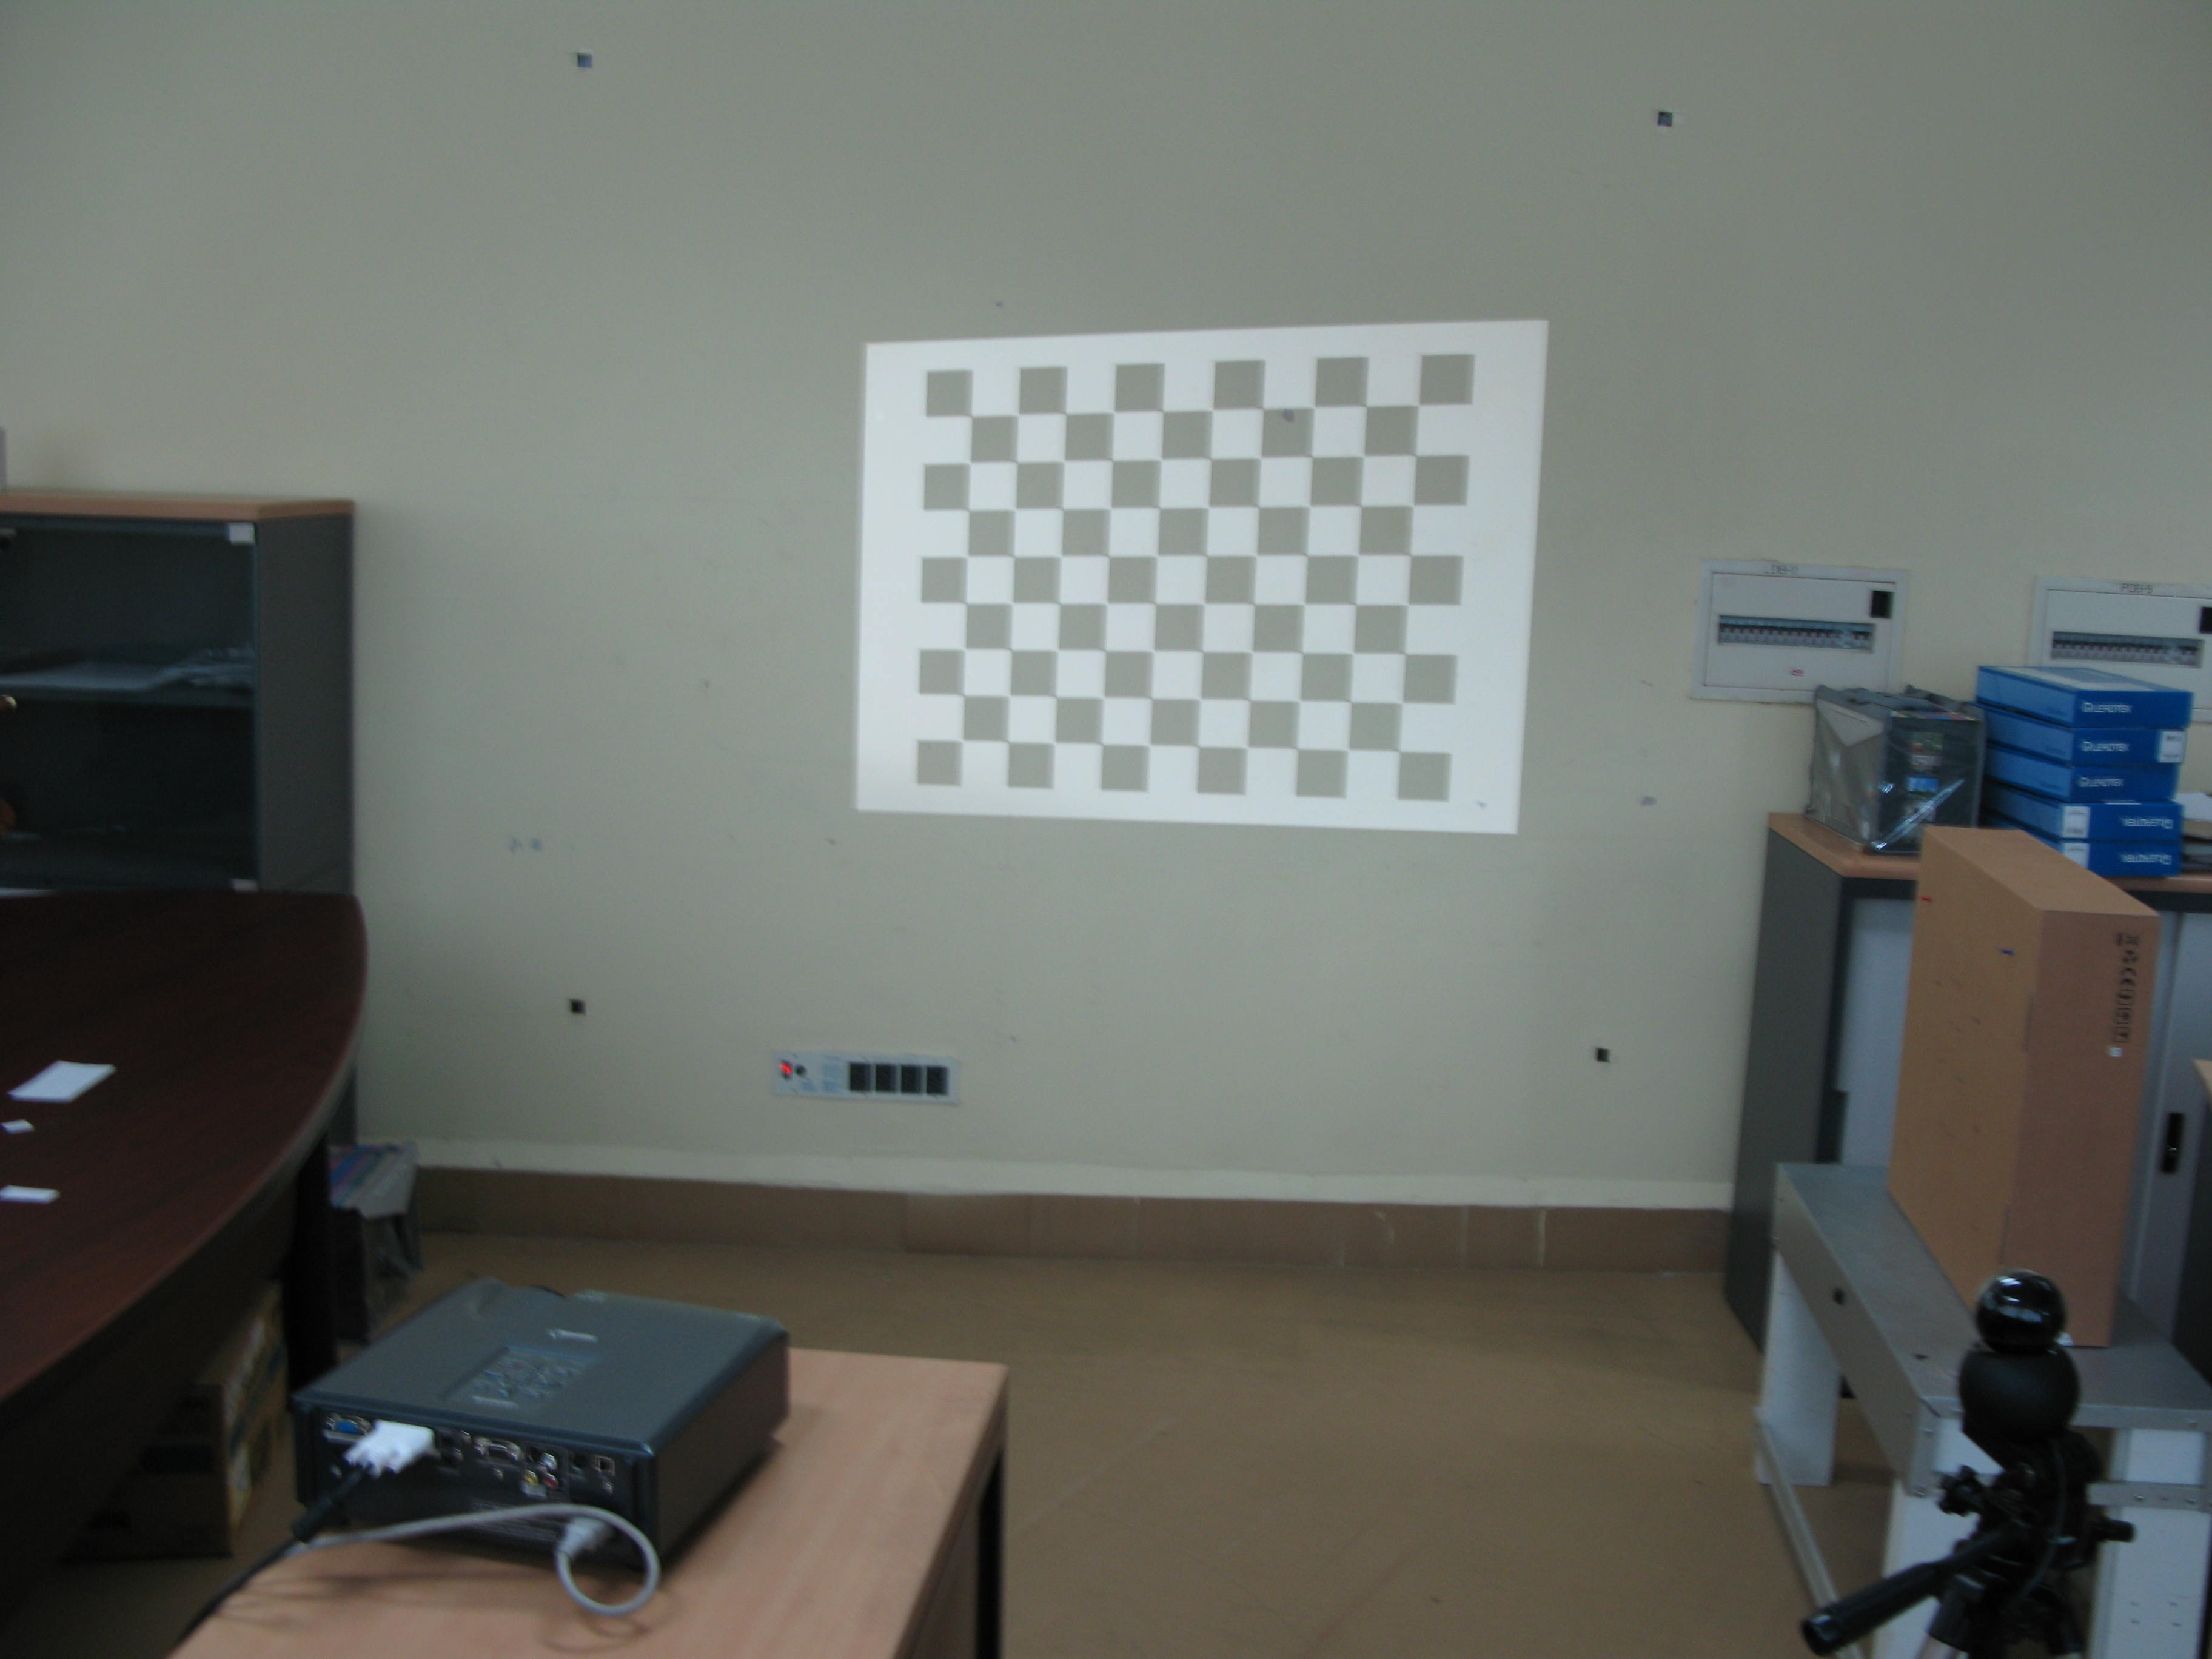
\includegraphics[width=7cm,height=5.5cm]{../img_source/system_extrinsic.jpg}  
\caption{Actual setup for extrinsic calibration}  
\label{fig:extrinsic_calib_setup}
\end{figure}  
  
\begin{figure}[!htbp]  
\centering  
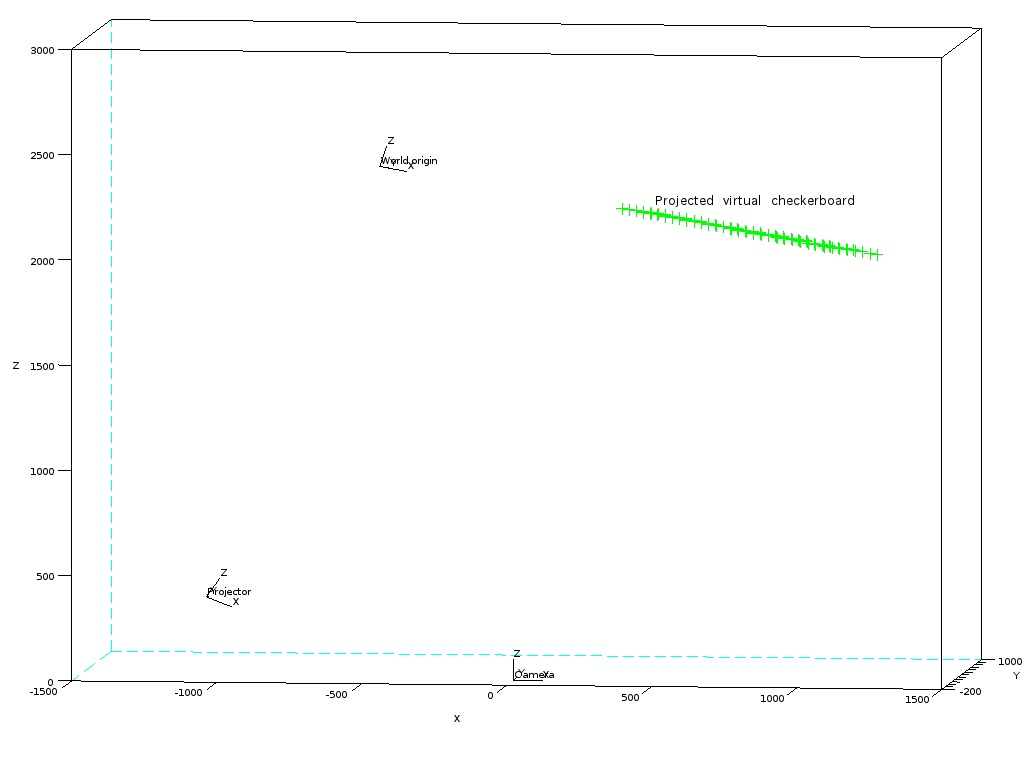
\includegraphics[width=17cm,height=11.3cm]{../img_source/system_plot_edit.jpg}  
\caption{Estimated system extrinsic geometry}  
\label{fig:extrinsic_plot}
\end{figure}  
\noindent  
 
  
\section{Discussion}  
During camera calibration it was observed that for larger distances($\sim2m$) of calibration board from camera, sub-pixel corner detection algorithm gives inaccurate results. Further, there has been no study on optimal \textit{window size} and \textit{termination criteria} for sub-pixel corner detection algorithm in the literature due to which these parameters were decided experimentally.\newline  
\indent Projector calibration using OpenCV camera calibration algorithm gives non-repeat-able estimated parameters of which reason is still unknown and deserves further study.\newline  
\indent It was observed that there are certain camera-projector geometric configurations for example when base-line between optical centers of camera and projector is small, for which OpenCV pose-estimation gives degenerate results, again this problem needs further study.   
  
  
\section{Summary}  
In this chapter, camera model was described as a series of transformations on a real world 3D point. In review, currently most popularly used calibration algorithms were briefly described. Further, working of the developed system calibration module was described with individual explanations of used procedure for camera, projector and relative extrinsic calibration. To make calibration results more comprehensive, individual plots for camera, projector and relative extrinsic calibration process were presented.
 


\appendix
\chapter{Tables}

\begin{table}
\caption{Armadillos}
\label{arm:table}
\begin{center}
\begin{tabular}{||l|l||}\hline
Armadillos & are \\\hline
our	   & friends \\\hline
\end{tabular}
\end{center}
\end{table}

\clearpage
\newpage

\chapter{Figures}

\vspace*{-3in}

\begin{figure}
\vspace{2.4in}
\caption{Armadillo slaying lawyer.}
\label{arm:fig1}
\end{figure}
\clearpage
\newpage

\begin{figure}
\vspace{2.4in}
\caption{Armadillo eradicating national debt.}
\label{arm:fig2}
\end{figure}
\clearpage
\newpage

%% This defines the bibliography file (main.bib) and the bibliography style.
%% If you want to create a bibliography file by hand, change the contents of
%% this file to a `thebibliography' environment.  For more information 
%% see section 4.3 of the LaTeX manual.
\begin{singlespace}
\begin{thebibliography}{10000000000}
\bibitem{1} %1
Microsoft Photosynth.\newline 
photosynth.net\newline
Accessed 3 December 2012

\bibitem{2} %2
Projective geometry tutorial.\newline 
http://www.cse.iitd.ernet.in/~suban/vision/tutorial/node1.html \newline
Accessed 4 December 2012

\bibitem{3} %3
Faugeras,Olivier.(1995).Stratification of 3-D vision: projective, affine, and metric representations,Journal of the Optical Society of America A,Vol-12,46548--4 


\bibitem{4} %4
Hartley,Richard I.,Sturm,Peter(1997).Triangulation, 
Computer Vision and Image Understanding,Volume 68, Issue 2, November 1997,Pages 146-157 

\bibitem{5}  %5
Saxena,Ashutosh,Sun,Min,Ng,Andrew Y.(2007).3-D Reconstruction from Sparse Views using Monocular Vision,ICCV workshop on Virtual Representations and Modeling of Large-scale environments (VRML),2007  

\bibitem{6} %#
Flexiscan3D scanner software \newline
http://www.3d3solutions.com/products/flexscan3d/ \newline
Accessed:3 December 2012

\bibitem{7} %#
Pan,B., Kemao,Q.,Huang,L.,and Asundi,A.(2009).Phase error analysis and compensation for nonsinusoidal waveforms in phase-shifting digital fringe projection profilometry, Opt. Lett.  34, 416-418. 

\bibitem{8} %#
Tsai,Roger Y. (1987) :A Versatile Camera Calibration Technique for High- 
Accuracy 3D Machine Vision Metrology Using Off-the-Shelf TV Cameras 
and Lenses,IEEE Journal of Robotics and Automation, Vol. RA-3, No. 4, 
August 1987, pp. 323-344. 

\bibitem{9} %#
Zhang,Song(2005).High-resolution, Real-time 3-D Shape Measurement,Ph.D. dissertation, Stony Brook University, Stony Brook, NY, 2005. 

\bibitem{10} %#
Zhang,Z.(2000).A flexible new technique for camera calibration. IEEE Transactions on Pattern Analysis and Machine Intelligence, 22(11):1330-1334, 2000 

\bibitem{11} %#
Vo,Minh,Wang,Zhaoyang,Pan,Bing,Pan,Tongyan(2012).Hyper-accurate flexible calibration technique for fringe-projection-based three-dimensional imaging,Opt. Express 20, 16926-16941 (2012) 

\bibitem{12} %#
Hartley,R.I.(1994),An algorithm for self calibration from several viewes.In Proceedings of IEEE Conference on Computer Vision and Pattern Recognition,pages 908-912,IEEE Computer Society Press 

\bibitem{13} %#
Luong,Q.~T,Faugeras,O.(1997).Self-calibration of a moving camera from point correspondences and fundamental matrices.The International Journal of Computer Vision,22(3):261-289,1997 

\bibitem{14} %#
Caprile,B,Torre,V.(1990).Using Vanishing Points for Camera Calibration.The International Journal Of Computer Vision,4(2):127-140,Mar.1990 

\bibitem{15} %#
Hartley,R.(1994).Self-calibration from multiple views with a rotating camera.In Proceedings of 3rd ECCV,volume 800-801 of 'Lecture notes in Computer Science' pages 471-478,Stockholm,Sweden,May 1994.Springer-Verlag 

\bibitem{16} %#
Zollner, Helmut and Sablatnig,Robert(2004).Comparison of Methods for Geometric Camera Calibration using Planar Calibration Targets,Proceedings of the 28th Workshop of the Austrian Association of Pattern Recognition, AAPR 2004,pp.237--244,OCG Schriftenreihe, {\"O}sterreichische Arbeitsgemeinschaft f{\"u}r Mustererkennung

\bibitem{17} %#
Heikkil\"{a},J.,Silven,O.(1997).A Four-Step Camera Calibration Procedure with Implicit Image Correction.
In Proc. of IEEE Computer Vision and Pattern Recognition, pp. 1106-1112, 1997

\bibitem{18} %#
Camera Calibration Toolbox For Matlab \newline
http://www.vision.caltech.edu/bouguetj/calib\_doc/index.html \newline
Accessed:3 December 2012 

\bibitem{19} %#
OpenCV documentation on Camera calibration \newline
http://docs.opencv.org/modules/calib3d/doc/calib3d.html \newline
Accessed 5 December 2012

\bibitem{20} %#
Levenberg Marquardt algorithm.\newline
http://en.wikipedia.org/wiki/Levenberg\%E2\%80\%93Marquardt\_algorithm \newline
Accessed 4 December 2012.

\bibitem{21} %# 
Extrinsic parameters estimation in OpenCV\newline 
http://opencv.willowgarage.com/documentation/camera\_calibration\_and\_3d\newline
\_reconstruction.html\#findextrinsiccameraparams2 \newline
Accessed 5 December 2012

\bibitem{22} %#
Bradski,Gary and Kaehler,Adrian(2008).Learning OpenCV,Computer Vision with the OpenCV Library.O'Reilly Media,September 2008 

\bibitem{23} %#
Asla Medeiros e Sa,Esdras Soares de Medeiros Filho,Paulo Cezar Carvalho,Luiz Velho.Coded Structured Light for 3D-photography:an Overview.\newline
www.visgraf.impa.br/Data/RefBib/PS\_PDF/rita-survey/survey.pdf \newline
Accessed 5 December 2012
  

\bibitem{24} %#
Salvi,J.,Pag\`es,J,Tutorial on Coded Light Projection techniques\newline 
http://eia.udg.es/~qsalvi/Tutorial\_Coded\_Light\_Projection\_Techniques\_arc\newline
hivos/v3\_document.html \newline
Accessed 4 December 2012

\bibitem{25} %#
Geng,J.(2011)."Structured-light 3D surface imaging: a tutorial," Adv. Opt. Photon.3, 128-160 .

\bibitem{26} %#
Pag\`es,Jordi,Salvi,Joaquim,Garcia,Rafael,Matabosch,Carles(2003).Overview of coded light projection techniques for automatic 3D profiling 

\bibitem{27} %#
Posdamer,J. L.,Altschuler,M. D.(1982). Surface measurement by 
space-encoded projected beam systems, Comput. Graph. Image Processing 
18(1), 1-17 (1982). 

\bibitem{28} %#
Inokuchi,S.,Sato,K.,Matsuda,F.(1984).Range-imaging for 3-D object recognition, 
in International Conference on Pattern Recognition (International 
Association for Pattern Recognition, 1984), pp. 806-808. 

\bibitem{29} %#
Caspi,D.,Kiryati,N.,Shamir,J.(1998),Range imaging with adaptive color 
structured light, IEEE Trans. Pattern Anal. Mach. Intell. 20(5), 470-480 
(May 1998). 

\bibitem{30} %#
Horn,Eli,Kiryati,Nahum(1997).Toward Optimal Structured Light Patterns,Image and Vision Computing,Vol. 17,pp.87-97 

\bibitem{31} %#
Ghiglia,Dennis C.,Pritt,Mark D..Two-Dimensional Phase Unwrapping: Theory, Algorithms, and Software.Wiley Publications,ISBN: 978-0-471-24935-1

\bibitem{32} %#
MacWilliams,F.J.,Sloane,N.J.A.(1976).Pseudorandom sequences and 
arrays, Proc. IEEE 64(12), 1715-1729. 

\bibitem{33} %#
De Bruijn sequnces\newline 
http://feed-back.be/nick/?page\_id=310\newline
Accessed 12 December 2012

\bibitem{34} %#
Moigne,J.Le,Waxman,A. M.(1985), Multi-resolution grid patterns for 
building range maps,in Vision-85, Applied Machine Vision Conference 
(ASME) (Society of Manufacturing Engineers, 1985), pp. 22-39. 

\bibitem{35} %#
Ulusoy,A. Osman,Calakli,F.,Taubin,G.(2009), One-shot scanning using De 
Bruijn spaced grids, in 2009 IEEE 12th International Conference on Computer 
Vision Workshops (ICCV Workshops) (IEEE, 2009), pp. 1786-1792. 
 
\bibitem{36} %#
Carrihill,B.,Hummel,R.(1985). Experiments with the intensity ratio depth sensor. In Computer Vision, Graphics and Image 
Processing, volume 32, pages 337--358. Academic Press, 1985 

\bibitem{37} %#
Chazan,G.,Kiryati,N.(1995). Pyramidal intensity ­ratio depth sensor. Technical report 121, Center for Communication and Informa­tion Technologies, Department of Electrical Engineering, Technion, Haifa, Israel, October 1995. 

\bibitem{38} %#
Hung,D.C.D.(1993). 3d scene modelling by sinusoid encoded illumination. Image and Vision Computing, 11:251--256, 1993. 

\bibitem{39} %#
Tajima,J.,Iwakawa,M.(1990). 3D data acquisition by rainbow range finder. In International Conference on Pattern Recognition, pages 309--313, 1990 

\bibitem{40} %#
Sato,T.(1999). Multispectral pattern projection range finder. In Proceedings of the Conference on ThreeDimensional Image Capture and Applications II, volume 3640, pages 28--37, San Jose, California, January 1999. SPIE. 

\bibitem{41} %#
Stripe boundary codes for real-time structured-light range scanning of moving 
objects. In The 8th IEEE International Conference on 
Computer Vision, pages II: 359-366, 2001. 

\bibitem{42} %#
Zhang,Song(2010).Recent progresses on real-time 3D shape measurement using digital fringe projection techniques.Optics and Lasers in Engineering, Volume 48, Issue 2, February 2010, Pages 149-158 

\bibitem{43} %#
Gorthi,S.S.,Rastogi,P(2009).Fringe projection technique:Whither we are?.Optics and Lasers in Engineering, 2009 

\bibitem{44} %#
`open-light'-Google code \newline
http://code.google.com/p/open-light/\newline
Accessed 5 December 2012 

\bibitem{45} %#
`Structured-light'-Goole code \newline
http://code.google.com/p/structured-light/ \newline
Accessed 5 December 2012

\bibitem{46} %#
Gupta,Mohit and Agrawal, Amit and Veeraraghavan, Ashok and Narasimhan, Srinivasa,G.(2012).A Practical Approach to 3D Scanning in the Presence of Interreflections,Subsurface Scattering and Defocus.International Journal of Computer Vision,pp.1-23,Springer

\bibitem{47} %#
Ghiglia,Dennis C.,Romero,Louis A.(1996)."Minimum Lp-norm two-dimensional phase unwrapping," J. Opt. Soc. Am. A 13, 1999-2013 (1996)

\bibitem{48} %#
Mundy,J.,Zisserman,A.(1992).Appendix:Projective geometry for machine vision-Geometric invariances in computer vision,MIT Press,1992 
 

\bibitem{49} %#
R.I.,Hartley,Zisserman,A.(2004).Multiple View Geometry in Computer Vision,Second edition,Cambridge University Press, ISBN:0521540518
  
\bibitem{50} %#
Hartley,R.,Gupta,R.,Chang,T.(1992).Stereo from uncalibrated cameras, 
in Proceedings, IEEE Conference on Computer Vision and Pattern Recognition, 1992, pp. 761-764. 

\bibitem{51} %#
Triangulation\newline 
http://en.wikipedia.org/wiki/Triangulation\newline
Accessed 5 December 2012

\bibitem{52} %#   
Brett R.,Jones(2010).AUGMENTING COMPLEX SURFACES WITH PROJECTOR-CAMERA SYSTEMS,M.S.Thesis,University of Illinois at Urbana-Champaign

\bibitem{53} %#
Point cloud library.\newline
pointclouds.org/.\newline
Accessed 24 November 2012

\bibitem{54} %#
Accuracy \& precision.\newline
http://en.wikipedia.org/wiki/Accuracy\_and\_precision\newline
Accessed 24 November 2012

\bibitem{55} %#
OpenCV function for checkerboard corner detection.\newline
http://opencv.willowgarage.com/documentation/camera\_calibration\_and\_3d\_\newline
reconstruction.html\#findchessboardcorners\newline
Accessed 24 November 2012

\bibitem{56} %#
Sansoni,G., Carocci,M., and Rodella,R.(1999). "Three-Dimensional Vision Based on a Combination of Gray-Code and Phase-Shift Light Projection: Analysis and Compensation of the Systematic Errors," Appl. Opt.  38, 6565-6573 .

\bibitem{57} %#
Microsoft Kinect.\newline
http://www.xbox.com/en-US/KINECT.\newline
Accessed 24 November 2012

\bibitem{58} %#
OpenNi home page.\newline
openni.org/.Accessed 24 November 2012

\bibitem{59} %#
OpenKinect home page.\newline
openkinect.org/.Accessed 24 November 2012

\bibitem{60} %#
RGBDemo program for accessing kinect data.\newline
labs.manctl.com/rgbdemo/ \newline
Accessed 24 November 2012

\bibitem{61} %#
Skanect for Windows \& Mac-plateform.\newline
http://manctl.com/products.html.\newline
Accessed 24 November 2012

\bibitem{62} %#
Code laboratory.\newline
http://codelaboratories.com/nui/.\newline 
Accessed 24 November 2012

\bibitem{63} %#
Khoshelham, K., Elberink, S.O.(2012). Accuracy and Resolution of Kinect Depth Data for Indoor Mapping Applications. Sensors, 12, 1437-1454.

\bibitem{64} %#
Freedman, B., Shpunt, A., Machline, M., \& Arieli, Y. (2010).
Patent No. US2010/0018123 A1. United States of America.

\bibitem{65} %#
Smisek, J., Jancosek, M., Pajdla, T., (2011), "3D with Kinect," Computer Vision Workshops (ICCV Workshops),pp.1154-1160, 6-13 Nov. 2011
doi: 10.1109/ICCVW.2011.6130380

\bibitem{66} %#
ifixit Kinect teardown.\newline
http://www.ifixit.com/Teardown/Microsoft+Kinect+Teardown/4066/1.\newline
Accessed 24 November 2012

\bibitem{67} %#
ROS kinect calibration page. \newline
http://www.ros.org/wiki/openni\_launch/Tutorials/IntrinsicCalibration?actio\newline
n=show\&redirect=openni\_camera\%2Fcalibration.\newline
Accessed 24 November 2012

\bibitem{68} %#
Moln\`ar,B., Toth,C.K., and Detrek\"{o}i,A.(2012). ACCURACY TEST OF MICROSOFT KINECT FOR HUMAN MORPHOLOGIC MEASUREMENTS, Int. Arch. Photogramm. Remote Sens. Spatial Inf. Sci., XXXIX-B3, 543-547, doi:10.5194/isprsarchives-XXXIX-B3-543-2012

\bibitem{69} %#
Herrera C.,D.,Kannala, J.,Heikkil\"{a},J.(2012).Joint depth and color camera calibration with distortion correction, TPAMI,.

\bibitem{70} %#
Boehm,J.(2012).NATURAL USER INTERFACE SENSORS FOR HUMAN BODY MEASUREMENT, Int. Arch. Photogramm. Remote Sens. Spatial Inf. Sci., XXXIX-B3, 531-536, doi:10.5194/isprsarchives-XXXIX-B3-531-2012

\bibitem{71} %#
Chow,J.C.K.,Ang,K.D.,Lichti,D.D.,and Teskey,W.F.(2012). 
PERFORMANCE ANALYSIS OF A LOW-COST TRIANGULATION-BASED 3D
CAMERA: MICROSOFT KINECT SYSTEM
International Archives of the Photogrammetry, Remote Sensing and Spatial Information Sciences, Volume XXXIX-B5
XXII ISPRS Congress

\bibitem{72} %#
Salvi,Joaquim,Armangu\`e,Xavier,Batlle,Joan(2002).A comparative review of camera calibrating methods with accuracy evaluation, Pattern Recognition, Volume 35, Issue 7, July 2002, Pages 1617-1635, ISSN 0031-3203, 10.1016/S0031-3203(01)00126-1.

\bibitem{73} %#
Drar\`eni, J. and  Roy, S. and Sturm, P.(2012).Methods for Geometrical Video Projector Calibration,Machine Vision and Applications

\end{thebibliography}
\end{singlespace}


\end{document}

